%% Volume I, Chapter 4: Counting and Discrete Structures
\chapter{Counting and Discrete Structures}
\label{ch:counting}

\abstract{How long will an algorithm run on the worst input? How likely is a run of bad luck? How surprising is an observed ranking if a treatment has no effect? Each of them becomes, sooner or later, a question of the form ``how many?'': how many comparisons, outcomes or orderings. The sets involved are far too large to be listed: twenty keys can arrive in $20!\approx2.4\times10^{18}$ orders, and a computer producing a billion of them per second would need $77$ years. Counting must therefore be done by reasoning rather than by enumeration. This chapter develops the principles that make this possible and introduces graphs and trees, the structures in which networks, data structures and sparse matrices are described.}

\Cref{ch:sets} defined the number of elements of a finite set by means of bijections and used a few rules of counting informally: that the sizes of disjoint sets add up, that a product of sets has the product of their sizes as its size, and that $m$ objects cannot be placed in fewer than $m$ places without two of them sharing a place. This chapter proves these rules and builds on them. Its subject is \term{enumerative combinatorics}, the art of counting finite sets without listing their elements, together with the first notions of \term{graph theory}, the study of objects joined in pairs.

The chapter has three parts. The first part, \cref{sec:counting-principles,sec:perm-comb,sec:binomial,sec:ie-pigeonhole}, establishes the basic principles (the sum rule, the product rule, counting by bijections and counting in two ways), applies them to arrangements and selections, studies the binomial coefficients that arise and proves the principle of inclusion and exclusion and the pigeonhole principle. The second part, \cref{sec:recurrences,sec:gf}, turns to sequences of counts. A count that depends on a parameter $n$ often satisfies a recurrence, and \cref{sec:recurrences} shows how to solve the simplest recurrences; \cref{sec:gf} packs a whole sequence into a single formal power series, the generating function, so that recurrences and counting problems become algebra. The third part, \cref{sec:graphs,sec:trees}, introduces graphs and trees. A final section, \cref{sec:counting-probability}, shows that probabilities in models with equally likely outcomes are ratios of counts.

The results of this chapter return throughout the series. The number of steps of an algorithm is a count (Volume~IV); the exact distribution of a rank statistic is a count of orderings (Volume~XIV); a sparse matrix is a graph with numbers on its edges (Volume~IX). As in the previous chapters, this is a review: every result is stated precisely, most are proved, and for the others we give the idea of the proof and a reference. Two topics that need analysis are deferred to Part~II: the growth of $n!$, described by Stirling's formula, and the precise behaviour of sums such as $1+\frac12+\cdots+\frac1n$; both are treated in \cref{ch:series}.

\section{Basic Counting Principles}
\label{sec:counting-principles}

Every count in this chapter rests on four principles. The \term{sum rule} counts a set by splitting it into disjoint parts; the \term{product rule} counts the outcomes of a sequence of choices; the \term{bijection principle} counts a set by matching it with a set already counted; and \term{double counting} counts one set in two ways and equates the results. This section states and proves them.

Recall from \cref{def:finite} that a set $A$ has $n$ elements, written $|A|=n$, if there is a bijection from $A$ to $\{0,1,\ldots,n-1\}$, and that this number is well defined by \cref{cor:finite}\,(i). Two sets have the same number of elements if and only if there is a bijection between them (\cref{prop:equinumerous}).

\subsection{The Sum Rule}

\begin{theorem}[Sum rule]
\label{thm:sum-rule}
Let $A$ and $B$ be finite sets with $A\cap B=\emptyset$. Then $A\cup B$ is finite and
\[
|A\cup B|=|A|+|B| .
\]
More generally, if $A_1,\ldots,A_k$ are finite sets that are \term{pairwise disjoint}, that is, $A_i\cap A_j=\emptyset$ whenever $i\ne j$, then
\[
|A_1\cup A_2\cup\cdots\cup A_k|=|A_1|+|A_2|+\cdots+|A_k| .
\]
\end{theorem}

\begin{proof}
Let $|A|=m$ and $|B|=n$, and let $f\colon A\to\{0,\ldots,m-1\}$ and $g\colon B\to\{0,\ldots,n-1\}$ be bijections. Define $h\colon A\cup B\to\{0,\ldots,m+n-1\}$ by $h(x)\coloneqq f(x)$ for $x\in A$ and $h(x)\coloneqq m+g(x)$ for $x\in B$. Since $A$ and $B$ are disjoint, every element of $A\cup B$ falls under exactly one of the two cases, so $h$ is a function. It numbers the elements of $A$ with $0,\ldots,m-1$ and those of $B$ with $m,\ldots,m+n-1$. It is injective: two elements of $A$ have different values because $f$ is injective, two elements of $B$ because $g$ is injective, and an element of $A$ and an element of $B$ because the first value is less than $m$ and the second is at least $m$. It is surjective: a number $j<m$ is $h(f^{-1}(j))$, and a number $j$ with $m\le j<m+n$ is $h(g^{-1}(j-m))$. Hence $|A\cup B|=m+n$.

The general statement follows by induction on $k$. For $k=1$ there is nothing to prove. If it holds for $k$ sets, let $A_1,\ldots,A_{k+1}$ be pairwise disjoint and put $U\coloneqq A_1\cup\cdots\cup A_k$. By the distributive law of \cref{thm:set-algebra}, $U\cap A_{k+1}=(A_1\cap A_{k+1})\cup\cdots\cup(A_k\cap A_{k+1})=\emptyset$. The first part and the inductive hypothesis give $|U\cup A_{k+1}|=|U|+|A_{k+1}|=|A_1|+\cdots+|A_k|+|A_{k+1}|$.
\end{proof}

The sum rule is the principle behind every argument of the form ``split into cases and add''. The proof of \cref{prop:product-size}, which counted the pairs in $A\times B$ row by row, and the proof of \cref{prop:power-set-size}, which split the subsets of a set into those that contain a given element and those that do not, both used it, and it is now justified. Two consequences are used constantly.

\begin{lemma}
\label{lem:subset-finite}
Let $A$ be a finite set with $|A|=n$ and let $B\subseteq A$. Then $B$ is finite, $|B|\le n$ and $|A\setminus B|=n-|B|$. Moreover, $|B|=n$ only if $B=A$.
\end{lemma}

\begin{proof}
We first prove by induction on $n$ that $B$ is finite with $|B|\le n$, and that $|B|=n$ only if $B=A$. For $n=0$ the set $A$ is empty, hence so is $B$. Suppose the claim holds for sets with $n$ elements, and let $|A|=n+1$. Choose a bijection $f\colon A\to\{0,\ldots,n\}$ and put $a\coloneqq f^{-1}(n)$. The restriction of $f$ to $A'\coloneqq A\setminus\{a\}$ is a bijection onto $\{0,\ldots,n-1\}$, so $|A'|=n$. The set $B'\coloneqq B\setminus\{a\}$ is a subset of $A'$, so by the inductive hypothesis it is finite with $|B'|\le n$. If $a\notin B$, then $B=B'$ and $|B|\le n<n+1$. If $a\in B$, then $B$ is the disjoint union of $B'$ and $\{a\}$, and the sum rule gives $|B|=|B'|+1\le n+1$; equality holds only if $|B'|=n$, that is, $B'=A'$ by the inductive hypothesis, and then $B=A'\cup\{a\}=A$.

Finally, $A$ is the disjoint union of $B$ and $A\setminus B$, both of which are finite by what we have just shown, so $n=|B|+|A\setminus B|$ by the sum rule.
\end{proof}

\begin{proposition}
\label{prop:union-two}
For finite sets $A$ and $B$,
\[
|A\cup B|=|A|+|B|-|A\cap B| .
\]
In particular $|A\cup B|\le|A|+|B|$, with equality if and only if $A$ and $B$ are disjoint.
\end{proposition}

\begin{proof}
The set $A\cup B$ is the disjoint union of $A$ and $B\setminus A$, and $B\setminus A=B\setminus(A\cap B)$. By the sum rule and \cref{lem:subset-finite}, $|A\cup B|=|A|+|B\setminus(A\cap B)|=|A|+|B|-|A\cap B|$. The last statement holds because $|A\cap B|=0$ exactly when $A\cap B=\emptyset$.
\end{proof}

For example, among the numbers $1,\ldots,100$ there are $50$ even numbers and $33$ multiples of $3$, by the rule $\lfloor n/b\rfloor$ for the number of multiples of $b$ (\cref{sec:division}). The numbers that are both are the multiples of $6$, of which there are $16$. So $50+33-16=67$ of the numbers are divisible by $2$ or by $3$, and $33$ are divisible by neither. \Cref{sec:ie-pigeonhole} extends the formula to any number of sets.

\subsection{The Product Rule}

Many counting problems describe the objects to be counted as the result of a sequence of choices. A licence plate consists of three letters followed by three digits; a password is a word of eight characters; a schedule assigns one of several slots to each of several tasks. The product rule counts such objects, and its precise form explains what may and what may not depend on earlier choices.

\begin{theorem}[Product rule]
\label{thm:product-rule}
Let $S$ be a set of $k$-tuples. For $0\le i\le k$ let $S_i$ be the set of \term{prefixes} of length $i$ of elements of $S$, that is, the set of $i$-tuples $(s_1,\ldots,s_i)$ for which there is an element $(s_1,\ldots,s_k)\in S$ that begins with them; thus $S_0$ contains only the empty tuple, and $S_k=S$. Suppose there are natural numbers $n_1,\ldots,n_k$ such that, for each $i=1,\ldots,k$, every prefix in $S_{i-1}$ can be extended to exactly $n_i$ prefixes in $S_i$. Then
\[
|S|=n_1n_2\cdots n_k .
\]
\end{theorem}

\begin{proof}
We show $|S_i|=n_1\cdots n_i$ by induction on $i$. For $i=0$, $|S_0|=1$, the empty product. Let $1\le i\le k$ and suppose $|S_{i-1}|=n_1\cdots n_{i-1}$. Every element of $S_i$ is an extension of exactly one element of $S_{i-1}$, namely of its own prefix of length $i-1$. Hence $S_i$ is the disjoint union, over the elements $p\in S_{i-1}$, of the sets of extensions of $p$, each of which has $n_i$ elements by hypothesis. By the sum rule, $|S_i|=n_i\,|S_{i-1}|=n_1\cdots n_i$. For $i=k$ this is the claim.
\end{proof}

The hypothesis is weaker than it may look: the \emph{set} of options for the $i$th component may depend on the earlier components, as long as their \emph{number} does not. For instance, the number of words of three different letters from an alphabet of $26$ letters is $26\cdot25\cdot24=15\,600$: there are $26$ choices for the first letter, then $25$ for the second, whichever letter was chosen first, and then $24$ for the third. The set of letters available for the second position depends on the first letter, but its size is always $25$. When the number of options does vary, the sum rule must be used instead. The pairs $(i,j)$ with $1\le i<j\le n$ cannot be counted by the product rule, since for a given $i$ there are $n-i$ choices of $j$; splitting by the value of $i$ and adding gives $(n-1)+(n-2)+\cdots+0=n(n-1)/2$, by \eqref{eq:sum-k}.

When the choices are independent, so that $S=A_1\times\cdots\times A_k$, the theorem reduces to $|A_1\times\cdots\times A_k|=|A_1|\cdots|A_k|$, which extends \cref{prop:product-size}. There are $26^3\cdot10^3=17\,576\,000$ licence plates of the form described above, and $2^{64}$ patterns of $64$ bits.

A sequence of choices can be drawn as a \term{decision tree}. Its root stands for the empty prefix, the points at depth $i$ stand for the elements of $S_i$, each point is joined to its extensions, and the points at the bottom, the leaves, stand for the elements of $S$. \Cref{fig:decision-tree} shows the decision tree for choosing a subset of $\{a,b,c\}$: for each of the three elements in turn we decide whether to include it. Every point has two extensions, and the tree has $2\cdot2\cdot2=8$ leaves. Trees of this kind are studied in their own right in \cref{sec:trees}.

\begin{figure}
\sdfloat{%
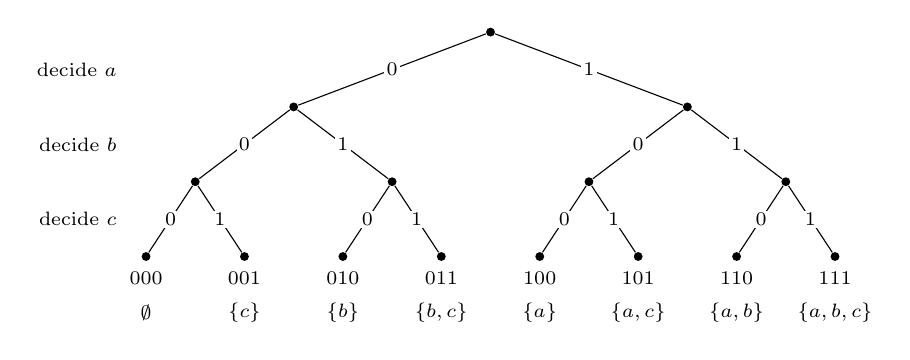
\begin{tikzpicture}[font=\scriptsize, x=1.25cm, y=0.95cm,
  dn/.style={circle, fill=black, inner sep=0pt, minimum size=3.2pt},
  de/.style={line width=0.4pt},
  el/.style={midway, fill=white, inner sep=0.8pt}]
\node[dn] (r) at (0,0) {};
\node[dn] (v0) at (-2,-1) {}; \node[dn] (v1) at (2,-1) {};
\draw[de] (r) -- node[el] {$0$} (v0); \draw[de] (r) -- node[el] {$1$} (v1);
\foreach \a in {0,1} {
  \foreach \b in {0,1} {
    \pgfmathsetmacro\x{4*\a-2+2*\b-1}
    \node[dn] (v\a\b) at (\x,-2) {};
    \draw[de] (v\a) -- node[el] {$\b$} (v\a\b);
    \foreach \c in {0,1} {
      \pgfmathsetmacro\xx{\x+\c-0.5}
      \node[dn] (v\a\b\c) at (\xx,-3) {};
      \draw[de] (v\a\b) -- node[el] {$\c$} (v\a\b\c);
      \node[below=2pt] at (v\a\b\c) {$\a\b\c$};}}}
\foreach \l/\x in {{\emptyset}/-3.5,{\{c\}}/-2.5,{\{b\}}/-1.5,{\{b,c\}}/-0.5,{\{a\}}/0.5,{\{a,c\}}/1.5,{\{a,b\}}/2.5,{\{a,b,c\}}/3.5}
  {\node at (\x,-3.75) {$\l$};}
\node[anchor=east] at (-3.7,-0.5) {decide $a$};
\node[anchor=east] at (-3.7,-1.5) {decide $b$};
\node[anchor=east] at (-3.7,-2.5) {decide $c$};
\end{tikzpicture}}{The decision tree for choosing a subset $S$ of $\{a,b,c\}$. At each level one element is decided: the label $1$ means that it is put into $S$, the label $0$ that it is left out. The eight leaves carry the binary words $\mathbf 1_S(a)\mathbf 1_S(b)\mathbf 1_S(c)$ and, below them, the corresponding subsets.\label{fig:decision-tree}}
\end{figure}

\subsection{Counting by Bijection}

By \cref{prop:equinumerous}, a set that is in bijection with a finite set of known size has that size too. This \term{bijection principle} is the most flexible counting tool: a set that is hard to count directly is matched with one that is easy to count. The number of subsets of a finite set illustrates both this principle and the product rule. \Cref{prop:power-set-size} proved by induction that a set of $n$ elements has $2^n$ subsets; here are two further proofs.

\emph{First proof, by bijection.} Let $A=\{a_1,\ldots,a_n\}$ with distinct $a_i$. The map that sends a subset $S\subseteq A$ to the binary word $\bigl(\mathbf 1_S(a_1),\ldots,\mathbf 1_S(a_n)\bigr)\in\{0,1\}^n$ is a bijection, since a subset is determined by which elements it contains and every word arises from the subset of the positions where it has a $1$. By \cref{prop:product-size}, $|\{0,1\}^n|=2^n$.

\emph{Second proof, by the product rule.} A subset is specified by deciding, for $a_1,\ldots,a_n$ in turn, whether to include it. Each decision has two outcomes, whatever the earlier decisions were, so there are $2^n$ subsets. \Cref{fig:decision-tree} shows the case $n=3$.

The same reasoning counts functions, and it makes precise the remark in \cref{sec:functions} that explains the notation $B^A$.

\begin{proposition}
\label{prop:functions-count}
Let $A$ and $B$ be finite sets with $|A|=m$ and $|B|=n$. Then the set $B^A$ of all functions from $A$ to $B$ has $n^m$ elements, with the convention $0^0=1$.
\end{proposition}

\begin{proof}
Write $A=\{a_1,\ldots,a_m\}$ with distinct $a_i$. The map $f\mapsto\bigl(f(a_1),\ldots,f(a_m)\bigr)$ is a bijection from $B^A$ to $B^m$: a function is determined by its values, and any $m$-tuple of values defines a function. By \cref{prop:product-size}, $|B^m|=n^m$ for $m\ge1$. For $m=0$ the domain is empty, and there is exactly one function from $\emptyset$ to $B$, the empty function, whose graph is the empty set; this agrees with $n^0=1$, also for $n=0$.
\end{proof}

For example, there are $2^{3}=8$ functions from a set of three elements to $\{0,1\}$, one for each subset, and $3^{2}=9$ functions from a set of two elements to a set of three. A program that maps each of $m$ inputs to one of $n$ output values, such as a hash function on a finite set of keys, is one of $n^m$ possibilities.

\subsection{Double Counting}

The fourth principle counts one set in two different ways. Since both counts give the size of the same set, they are equal, and the resulting equation is often far from obvious. This method is also called \term{counting in two ways}~\cite{aigner2018proofs,vanlint2001}.

\begin{proposition}[Double counting]
\label{prop:double-counting}
Let $A$ and $B$ be finite sets and $R\subseteq A\times B$ a relation. For $a\in A$ let $r(a)$ be the number of $b\in B$ with $(a,b)\in R$, and for $b\in B$ let $c(b)$ be the number of $a\in A$ with $(a,b)\in R$. Then
\[
\sum_{a\in A}r(a)=|R|=\sum_{b\in B}c(b).
\]
\end{proposition}

\begin{proof}
The set $R$ is the disjoint union, over $a\in A$, of the sets $\{(a,b): (a,b)\in R\}$, which have $r(a)$ elements; the sum rule gives the first equation. Splitting $R$ according to the second component gives the second.
\end{proof}

In the matrix picture of a relation (\cref{fig:relation}B), $r(a)$ is the number of ones in row $a$ and $c(b)$ the number of ones in column $b$: adding the row sums and adding the column sums both count all the ones of the matrix. Here is a first application. For a positive integer $n$ let $\tau(n)$ be the number of positive divisors of $n$. Counting the pairs $(k,n)$ with $1\le k,n\le N$ and $k\mid n$ first by $n$ and then by $k$ gives
\begin{equation}
\sum_{n=1}^{N}\tau(n)=\sum_{k=1}^{N}\Bigl\lfloor\frac Nk\Bigr\rfloor ,
\label{eq:divisor-sum}
\end{equation}
because, for a fixed $k$, the numbers $n\le N$ divisible by $k$ are the $\lfloor N/k\rfloor$ multiples $k,2k,\ldots$ of $k$ (\cref{sec:division}). For $N=10$ the left side is $1+2+2+3+2+4+2+4+3+4=27$ and the right side is $10+5+3+2+2+1+1+1+1+1=27$. The function $\tau$ jumps around irregularly, while the right side is easy to estimate: since $\lfloor N/k\rfloor\le N/k$, the average of $\tau(1),\ldots,\tau(N)$ is at most $1+\frac12+\cdots+\frac1N$, a sum that grows only like the natural logarithm of $N$ (\cref{ch:series}). A typical number has few divisors, a fact that is far from evident when one looks at the divisors one number at a time.

\section{Permutations and Combinations}
\label{sec:perm-comb}

The most common counting problems ask in how many ways $k$ objects can be chosen from $n$. The answer depends on two questions: does the order of the chosen objects matter, and may an object be chosen more than once? The four combinations of the answers lead to four counting formulas, collected in \cref{tab:four-ways} at the end of the section.

\subsection{Arrangements and Permutations}

If the order matters and repetition is allowed, a choice of $k$ objects from a set $A$ of $n$ is a $k$-tuple in $A^k$, and there are $n^k$ of them. If repetition is not allowed, the count involves a product of decreasing factors.

\begin{definition}[Falling factorial]
\label{def:falling-factorial}
For a real number $x$ and $k\in\mathbb N$, the \term{falling factorial} is
\[
x^{\underline k}\coloneqq x(x-1)(x-2)\cdots(x-k+1)=\prod_{j=0}^{k-1}(x-j),
\]
read ``$x$ to the $k$ falling''; in particular $x^{\underline 0}=1$.
\end{definition}

For a natural number $n$, $n^{\underline n}=n!$, and $n^{\underline k}=n!/(n-k)!$ for $k\le n$. If $k>n$, the product contains the factor $n-n=0$, so $n^{\underline k}=0$. The notation, with the line under the exponent, was popularised by Graham, Knuth and Patashnik~\cite[Sect.~2.6]{graham1994concrete}; older texts write $(n)_k$.

\begin{theorem}[Arrangements]
\label{thm:arrangements}
Let $A$ be a set with $n$ elements and $k\in\mathbb N$. The number of $k$-tuples of pairwise distinct elements of $A$, called \term{$k$-arrangements} of $A$, is $n^{\underline k}$. Equivalently, there are $n^{\underline k}$ injections from a set of $k$ elements to $A$. In particular, a set of $n$ elements has $n!$ permutations.
\end{theorem}

\begin{proof}
Apply the product rule to the set $S$ of $k$-arrangements. A prefix $(s_1,\ldots,s_{i-1})$ consists of $i-1$ distinct elements, and it extends by any of the $n-(i-1)$ elements not among them, so $n_i=n-i+1$. If $i-1=n$, this number is $0$, and the product rule correctly gives $0$ arrangements for $k>n$. Hence $|S|=n(n-1)\cdots(n-k+1)=n^{\underline k}$. If $C=\{c_1,\ldots,c_k\}$ has $k$ elements, the map $f\mapsto(f(c_1),\ldots,f(c_k))$ is a bijection from the injections $C\to A$ to the $k$-arrangements, since $f$ is injective exactly when its values are distinct. Finally, a permutation of $A$ is a bijection $A\to A$; by \cref{cor:finite}\,(iii), the bijections $A\to A$ are exactly the injections $A\to A$, of which there are $n^{\underline n}=n!$.
\end{proof}

The theorem also counts the orders in which $n$ distinct items can be listed: $n!$. This number grows very fast. There are $3!=6$ orders of three items, $10!=3\,628\,800$ orders of ten, and
\[
20!=2\,432\,902\,008\,176\,640\,000\approx2.43\times10^{18}
\]
orders of twenty. A signed $64$-bit integer holds values up to $2^{63}-1\approx9.22\times10^{18}$, so $20!$ is the largest factorial that fits; $21!\approx5.11\times10^{19}$ overflows, and so does every larger factorial. For the same reason, a sorting algorithm cannot try all orders of its input, and an algorithm that sorts by comparisons must, in the worst case, make enough comparisons to distinguish $n!$ possibilities; \cref{sec:trees} turns this remark into a lower bound.

\subsection{Combinations and Binomial Coefficients}

If the order does not matter and repetition is not allowed, a choice of $k$ objects from $A$ is a $k$-element subset of $A$.

\begin{definition}[Binomial coefficient]
\label{def:binomial}
For a set $S$ and $k\in\mathbb N$, let $\binom Sk$ denote the set of $k$-element subsets of $S$. For $n,k\in\mathbb N$, the \term{binomial coefficient} $\binom nk$, read ``$n$ choose $k$'', is the number of $k$-element subsets of a set with $n$ elements.
\end{definition}

The number does not depend on which set of $n$ elements is used: a bijection $f\colon A\to A'$ maps the $k$-element subsets of $A$ bijectively to those of $A'$, by $T\mapsto f(T)$. The $k$-element subsets are also called \term{$k$-combinations}. For example, the $2$-element subsets of $\{a,b,c,d\}$ are
\[
\{a,b\},\ \{a,c\},\ \{a,d\},\ \{b,c\},\ \{b,d\},\ \{c,d\},
\]
so $\binom42=6$. Directly from the definition, $\binom n0=\binom nn=1$, $\binom n1=n$, and $\binom nk=0$ for $k>n$ by \cref{lem:subset-finite}.

\begin{theorem}
\label{thm:binomial-formula}
For all $n,k\in\mathbb N$,
\[
\binom nk=\frac{n^{\underline k}}{k!},\qquad\text{and}\qquad\binom nk=\frac{n!}{k!\,(n-k)!}\quad\text{if }k\le n .
\]
\end{theorem}

\begin{proof}
Let $A$ have $n$ elements. Every $k$-arrangement $(s_1,\ldots,s_k)$ of $A$ determines the $k$-element subset $\{s_1,\ldots,s_k\}$ of its entries. For a fixed $T\in\binom Ak$, the arrangements with set of entries $T$ are exactly the arrangements of all $k$ elements of $T$, of which there are $k!$ by \cref{thm:arrangements}. So the $n^{\underline k}$ arrangements fall into $\binom nk$ disjoint groups of $k!$ each, and the sum rule gives $n^{\underline k}=\binom nk\,k!$. The second formula follows from $n^{\underline k}=n!/(n-k)!$.
\end{proof}

The proof is an instance of a pattern worth remembering, the \term{division principle}: if a set of $N$ objects falls into groups of equal size $g$, then there are $N/g$ groups. Here the objects are arrangements, the groups are the arrangements with the same entries, and $g=k!$. For example,
\[
\binom{52}{5}=\frac{52\cdot51\cdot50\cdot49\cdot48}{5\cdot4\cdot3\cdot2\cdot1}=2\,598\,960
\]
is the number of hands of five cards from a deck of $52$. In a computation, the formula $n^{\underline k}/k!$ is preferable to $n!/(k!\,(n-k)!)$, which forms large intermediate factorials; better still, the product $\prod_{j=1}^{k}(n-k+j)/j$ can be accumulated from left to right, since after $j$ factors it equals $\binom{n-k+j}{j}$ and is therefore an integer at every step.

The formula $x^{\underline k}/k!$ makes sense for every real $x$, and this extension is useful in \cref{sec:gf}.

\begin{definition}[Binomial coefficients with general upper index]
\label{def:binomial-general}
For a real number $r$ and an integer $k$, put
\[
\binom rk\coloneqq\frac{r^{\underline k}}{k!}=\frac{r(r-1)\cdots(r-k+1)}{k!}\quad\text{if }k\ge0,\qquad\binom rk\coloneqq0\quad\text{if }k<0 .
\]
\end{definition}

By \cref{thm:binomial-formula}, this agrees with \cref{def:binomial} when $r$ and $k$ are natural numbers. For example, $\binom{1/2}{2}=\frac12\cdot\bigl(-\frac12\bigr)/2=-\frac18$ and $\binom{-1}{k}=(-1)(-2)\cdots(-k)/k!=(-1)^k$. More generally, for $n\in\mathbb N$, reversing the order of the factors gives the rule of \term{upper negation},
\begin{align}
\binom{-n}{k}&=\frac{(-n)(-n-1)\cdots(-n-k+1)}{k!}\notag\\
&=(-1)^k\frac{(n+k-1)\cdots(n+1)n}{k!}=(-1)^k\binom{n+k-1}{k} .
\label{eq:upper-negation}
\end{align}

\subsection{Multisets}

If the order does not matter but repetition is allowed, a choice of $k$ objects from $A$ is a collection in which an element may occur several times, like the coins in a purse or the letters of a word regardless of their order.

\begin{definition}[Multiset]
\label{def:multiset}
A \term{multiset} of size $k$ on a set $A$ is a function $\mu\colon A\to\mathbb N$ with $\sum_{a\in A}\mu(a)=k$. The number $\mu(a)$ is the \term{multiplicity} of $a$.
\end{definition}

For example, the purse with two coins of $1$ unit, one of $2$ and four of $5$ is the multiset $\mu$ on $\{1,2,5\}$ with $\mu(1)=2$, $\mu(2)=1$, $\mu(5)=4$; its size is $7$. If $A=\{a_1,\ldots,a_n\}$, a multiset of size $k$ on $A$ is the same as a solution $(x_1,\ldots,x_n)\in\mathbb N^n$ of the equation
\begin{equation}
x_1+x_2+\cdots+x_n=k ,
\label{eq:compositions}
\end{equation}
with $x_i=\mu(a_i)$.

\begin{theorem}[Stars and bars]
\label{thm:multisets}
Let $n\ge1$ and $k\in\mathbb N$. The number of multisets of size $k$ on a set of $n$ elements, which is also the number of solutions of \eqref{eq:compositions} in natural numbers, is
\[
\binom{n+k-1}{k}=\binom{n+k-1}{n-1}.
\]
\end{theorem}

\begin{proof}
Encode a solution $(x_1,\ldots,x_n)$ as a word of $k$ stars and $n-1$ bars: $x_1$ stars, a bar, $x_2$ stars, a bar, and so on, ending with $x_n$ stars. The word has length $n+k-1$. Conversely, every word of $k$ stars and $n-1$ bars arises from exactly one solution: the $n-1$ bars cut the word into $n$ (possibly empty) runs of stars, and $x_i$ is the length of the $i$th run. This is a bijection, and a word is determined by the set of the $k$ positions, among $n+k-1$, that hold stars. Hence there are $\binom{n+k-1}{k}$ words. The second form follows from the symmetry $\binom NK=\binom N{N-K}$, which holds because the complement $T\mapsto\{1,\ldots,N\}\setminus T$ is a bijection from the $K$-element subsets of $\{1,\ldots,N\}$ to the $(N-K)$-element subsets (\cref{lem:subset-finite}).
\end{proof}

\Cref{fig:stars-bars}A shows the encoding of the purse above, with the $n=3$ coin values and $k=7$ coins, as well as a solution of \eqref{eq:compositions} with $n=4$. The theorem has many disguises. The number of monomials $x_1^{e_1}\cdots x_n^{e_n}$ of total degree $k$ in $n$ variables is $\binom{n+k-1}{k}$; for instance there are $\binom42=6$ monomials of degree $2$ in three variables, namely $x^2$, $y^2$, $z^2$, $xy$, $xz$ and $yz$. The number of ways to distribute $k$ identical items into $n$ boxes is $\binom{n+k-1}{k}$. And the number of solutions of \eqref{eq:compositions} in \emph{positive} integers, which are called the \term{compositions} of $k$ into $n$ parts, is $\binom{k-1}{n-1}$ for $k\ge1$: substituting $x_i=y_i+1$ turns them into the solutions of $y_1+\cdots+y_n=k-n$ in natural numbers, of which there are $\binom{k-1}{n-1}$ by the theorem (and none if $k<n$).

\begin{figure}
\tikzset{star/.style={circle, fill=black, inner sep=0pt, minimum size=4.2pt},
  bar/.style={line width=0.9pt}}
\sdpanel{A}{\begin{tikzpicture}[font=\scriptsize, x=0.42cm]
\foreach \p in {1,2,4,6,7,8,9} {\node[star] at (\p,0.6) {};}
\foreach \p in {3,5} {\draw[bar] (\p,0.3) -- (\p,0.9);}
\node[anchor=west] at (10,0.6) {$(2,1,4)$};
\foreach \p in {1,2,4,7,8,9,10} {\node[star] at (\p,-0.35) {};}
\foreach \p in {3,5,6} {\draw[bar] (\p,-0.65) -- (\p,-0.05);}
\node[anchor=west] at (11,-0.35) {$(2,1,0,4)$};
\foreach \p in {1,...,10} {\node[black!60] at (\p,-0.95) {$\p$};}
\end{tikzpicture}}\hfill
\sdpanel{B}{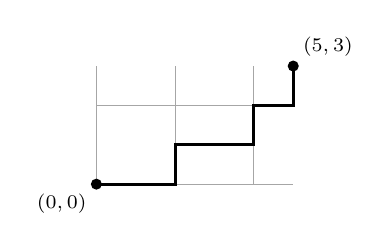
\begin{tikzpicture}[font=\scriptsize, x=0.5cm, y=0.5cm]
\draw[black!35, line width=0.3pt] (0,0) grid (5,3);
\draw[line width=1.1pt] (0,0) -- (2,0) -- (2,1) -- (4,1) -- (4,2) -- (5,2) -- (5,3);
\fill (0,0) circle (2pt); \fill (5,3) circle (2pt);
\node[below left] at (0,0) {$(0,0)$};
\node[above right] at (5,3) {$(5,3)$};
\end{tikzpicture}}
\caption{Two bijections with words. (A) Stars and bars: the multiset with multiplicities $(2,1,4)$ is the word of $7$ stars and $2$ bars in the upper row; the solution $(2,1,0,4)$ of $x_1+x_2+x_3+x_4=7$ is the word of $7$ stars and $3$ bars in the lower row, where two adjacent bars enclose an empty run. The grey numbers are the positions $1,\ldots,10$. (B) A lattice path from $(0,0)$ to $(5,3)$ with unit steps to the right ($R$) and upwards ($U$); it is the word $RRURRURU$, and it is determined by the positions $3$, $6$ and $8$ of its upward steps.}
\label{fig:stars-bars}
\end{figure}

A closely related count concerns paths on a grid, which will be needed in \cref{sec:recurrences} and which reappears in the exact distributions of rank statistics in Volume~XIV. A \term{lattice path} from $(0,0)$ to $(m,n)$, for $m,n\in\mathbb N$, is a sequence of points of $\mathbb Z^2$ that starts at $(0,0)$, ends at $(m,n)$ and moves at each step either one unit to the right or one unit upwards (\cref{fig:stars-bars}B).

\begin{proposition}
\label{prop:lattice-paths}
The number of lattice paths from $(0,0)$ to $(m,n)$ is $\binom{m+n}{m}$.
\end{proposition}

\begin{proof}
Every such path has exactly $m$ steps to the right and $n$ steps upwards, hence $m+n$ steps in all, and it is determined by the word in the letters $R$ and $U$ that lists its steps. Conversely, every word of $m$ letters $R$ and $n$ letters $U$ describes a path from $(0,0)$ to $(m,n)$. Such a word is determined by the set of positions of its $m$ letters $R$, a subset of $\{1,\ldots,m+n\}$ with $m$ elements, and there are $\binom{m+n}{m}$ of these.
\end{proof}

\subsection{Multinomial Coefficients}

The binomial coefficient $\binom nk$ also counts the ways of splitting a set of $n$ elements into two labelled parts, one of size $k$ and the other of size $n-k$. Splitting into more parts leads to the multinomial coefficients.

\begin{theorem}[Multinomial coefficients]
\label{thm:multinomial}
Let $k_1,\ldots,k_m\in\mathbb N$ with $k_1+\cdots+k_m=n$, and let $A$ be a set of $n$ elements. The number of tuples $(B_1,\ldots,B_m)$ of pairwise disjoint subsets of $A$ with $|B_i|=k_i$ for each $i$ (and hence with union $A$) is the \term{multinomial coefficient}
\[
\binom{n}{k_1,k_2,\ldots,k_m}\coloneqq\frac{n!}{k_1!\,k_2!\cdots k_m!}.
\]
The same number counts the words of length $n$ that contain the letter $\ell_i$ exactly $k_i$ times, for given distinct letters $\ell_1,\ldots,\ell_m$.
\end{theorem}

\begin{proof}
Apply the product rule to the tuples $(B_1,\ldots,B_m)$. After $B_1,\ldots,B_{i-1}$ have been chosen, $n-k_1-\cdots-k_{i-1}$ elements remain, and $B_i$ is any $k_i$-element subset of them, so
\[
n_i=\binom{n-k_1-\cdots-k_{i-1}}{k_i}=\frac{(n-k_1-\cdots-k_{i-1})!}{k_i!\,(n-k_1-\cdots-k_i)!}.
\]
In the product $n_1\cdots n_m$ the factorials $(n-k_1-\cdots-k_i)!$ for $i=1,\ldots,m-1$ cancel, and the last one is $(n-n)!=0!=1$; what remains is $n!/(k_1!\cdots k_m!)$. A word with the given letter counts corresponds to the tuple in which $B_i$ is the set of positions in $\{1,\ldots,n\}$ that hold the letter $\ell_i$, and this correspondence is a bijection.
\end{proof}

For $m=2$ the multinomial coefficient $\binom{n}{k,\,n-k}$ is the binomial coefficient $\binom nk$. For example, the letters of the word MISSISSIPPI, one M, four I, four S and two P, can be arranged in
\[
\binom{11}{1,4,4,2}=\frac{11!}{1!\,4!\,4!\,2!}=34\,650
\]
ways. Another way to see the formula is the division principle again: the $11!$ arrangements of eleven labelled letters fall into groups of $1!\,4!\,4!\,2!$ arrangements that differ only in the order of equal letters, and these groups give the same word.

\Cref{tab:four-ways} summarises the four ways of choosing. Volume~III uses these formulas when it builds probability models from equally likely outcomes, and \cref{sec:counting-probability} gives a first look at this use.

\begin{table}
\sdfloat{%
\begin{sdtable}{colspec={llll}, row{1}={font=\small\bfseries}}
\toprule
Order & Repetition & Number & $n=4$, $k=2$ \\
\midrule
matters & allowed & $n^k$ & $16$ \\
matters & not allowed & $n^{\underline k}=n(n-1)\cdots(n-k+1)$ & $12$ \\
does not matter & not allowed & $\binom nk$ & $6$ \\
does not matter & allowed & $\binom{n+k-1}{k}$ & $10$ \\
\bottomrule
\end{sdtable}}{The number of ways of choosing $k$ objects from a set of $n$. The four rows count, in order, the $k$-tuples, the $k$-arrangements, the $k$-element subsets and the multisets of size $k$. The last column lists the choices of two letters from $\{a,b,c,d\}$; for instance, the $10$ multisets are the $6$ subsets of two letters together with the $4$ doubled letters $aa,\ldots,dd$.\label{tab:four-ways}}
\end{table}

\section{The Binomial Theorem and Identities}
\label{sec:binomial}

The binomial coefficients satisfy a large number of identities, and most of them can be proved in two ways: by algebra, or by showing that both sides count the same set. The combinatorial proofs are usually shorter and always more illuminating, since they explain \emph{why} an identity holds. This section presents the identities that are used most often, the binomial theorem that gives the coefficients their name, and estimates of their size.

\subsection{Pascal's Triangle}

\begin{proposition}
\label{prop:pascal}
For all $n\in\mathbb N$ and all integers $k$:
\begin{enumerate}
\item $\binom nk=\binom n{n-k}$ \quad(symmetry);
\item $\binom nk=\binom{n-1}{k-1}+\binom{n-1}{k}$ if $n\ge1$ \quad(Pascal's rule).
\end{enumerate}
\end{proposition}

\begin{proof}
(i) If $0\le k\le n$, taking complements is a bijection from the $k$-element subsets of a set $A$ of $n$ elements to its $(n-k)$-element subsets, as in the proof of \cref{thm:multisets}. If $k<0$ or $k>n$, both sides are $0$.

(ii) Let $A$ have $n\ge1$ elements and fix $a\in A$. The $k$-element subsets of $A$ fall into two disjoint groups. Those that do not contain $a$ are the $k$-element subsets of $A\setminus\{a\}$, and there are $\binom{n-1}{k}$ of them. Those that contain $a$ are the sets $T\cup\{a\}$ with $T$ a $(k-1)$-element subset of $A\setminus\{a\}$, and there are $\binom{n-1}{k-1}$ of them. The sum rule gives the identity for $0\le k\le n$, and for other $k$ both sides are $0$ (for $k=0$ the right side is $0+1$, for $k=n$ it is $1+0$).
\end{proof}

Pascal's rule computes all binomial coefficients from $\binom00=1$ by additions alone. Writing the coefficients $\binom nk$ in rows, $n=0,1,2,\ldots$, each entry is the sum of the two entries above it. The result is \term{Pascal's triangle}, shown in \cref{fig:pascal}. It is named after Blaise Pascal, whose \emph{Trait\'e du triangle arithm\'etique} was published in 1665~\cite{pascal1665}, but the triangle was known centuries earlier in China, India and Persia~\cite{edwards1987pascal}. The triangle displays many of the identities of this section: its rows are symmetric by \cref{prop:pascal}\,(i), and their sums are the powers of $2$.

\begin{figure}
\sdfloat{%
\begin{tikzpicture}[font=\scriptsize, x=0.78cm, y=0.56cm]
\foreach \n/\k in {2/2,3/2,4/2,5/2,6/2} {\fill[sdfill] ({(\k-0.5*\n)},{-\n}) circle (0.36);}
\draw[line width=0.6pt] ({3-3.5},-7) circle (0.36);
\draw[-{Latex[length=1.2mm]}, line width=0.4pt] ({3-2.5+0.12},{-5-0.25}) -- ({4-3-0.1},{-6+0.28});
\draw[-{Latex[length=1.2mm]}, line width=0.4pt] ({4-2.5-0.12},{-5-0.25}) -- ({4-3+0.1},{-6+0.28});
\foreach \row [count=\n from 0] in {{1},{1,1},{1,2,1},{1,3,3,1},{1,4,6,4,1},{1,5,10,10,5,1},{1,6,15,20,15,6,1},{1,7,21,35,35,21,7,1},{1,8,28,56,70,56,28,8,1}} {
  \node[black!60, anchor=east] at (-5.2,-\n) {$n=\n$};
  \foreach \v [count=\k from 0] in \row {\node at ({\k-0.5*\n},{-\n}) {$\v$};}}
\end{tikzpicture}}{Pascal's triangle, rows $n=0,\ldots,8$; the entries of row $n$ are $\binom n0,\ldots,\binom nn$. Each entry is the sum of the two entries above it, as the arrows show for $\binom64=\binom53+\binom54=10+5$. The shaded entries $\binom22,\ldots,\binom62$ add up to the circled entry $\binom73=35$ (\cref{prop:hockey-stick}).\label{fig:pascal}}
\end{figure}

\subsection{The Binomial Theorem}

\begin{theorem}[Binomial theorem]
\label{thm:binomial}
Let $x$ and $y$ be elements of a commutative ring, for instance real or complex numbers, and let $n\in\mathbb N$. Then
\[
(x+y)^n=\sum_{k=0}^{n}\binom nk x^ky^{n-k}.
\]
\end{theorem}

\begin{proof}
By induction on $n$. For $n=0$ both sides equal $1$. Suppose the formula holds for $n$. Then, by the distributive law,
\[
(x+y)^{n+1}=(x+y)\sum_{k=0}^{n}\binom nk x^ky^{n-k}=\sum_{k=0}^{n}\binom nk x^{k+1}y^{n-k}+\sum_{k=0}^{n}\binom nk x^ky^{n+1-k}.
\]
In the first sum we replace $k$ by $k-1$, so that it becomes $\sum_{k=1}^{n+1}\binom n{k-1}x^ky^{n+1-k}$. Since $\binom n{-1}=0$ and $\binom n{n+1}=0$, both sums may be taken over $k=0,\ldots,n+1$, and Pascal's rule gives
\[
(x+y)^{n+1}=\sum_{k=0}^{n+1}\Bigl(\binom n{k-1}+\binom nk\Bigr)x^ky^{n+1-k}=\sum_{k=0}^{n+1}\binom{n+1}{k}x^ky^{n+1-k}.
\]
\end{proof}

There is also a combinatorial proof, which explains why binomial coefficients appear. Expand the product $(x+y)(x+y)\cdots(x+y)$ of $n$ factors by the distributive law without collecting terms. The result is a sum of $2^n$ products, one for each way of choosing either $x$ or $y$ from every factor. A choice that takes $x$ from exactly $k$ of the factors, and $y$ from the others, produces the term $x^ky^{n-k}$, and such a choice is determined by the set of the $k$ factors that contribute $x$. There are $\binom nk$ such sets, hence $\binom nk$ terms equal to $x^ky^{n-k}$. For $n=3$, for instance, the eight products are $xxx$, $xxy$, $xyx$, $yxx$, $xyy$, $yxy$, $yyx$ and $yyy$, and collecting them gives $x^3+3x^2y+3xy^2+y^3$. The commutativity of the ring is needed to identify $xxy$, $xyx$ and $yxx$; for square matrices, which do not commute, the binomial theorem is false in general (Part~III).

Substituting particular values for $x$ and $y$ yields a family of identities.

\begin{corollary}
\label{cor:binomial-sums}
For every $n\in\mathbb N$:
\begin{enumerate}
\item $\sum_{k=0}^{n}\binom nk=2^n$;
\item $\sum_{k=0}^{n}(-1)^k\binom nk=0$ if $n\ge1$;
\item $k\binom nk=n\binom{n-1}{k-1}$ for all integers $k$, if $n\ge1$ \quad(absorption);
\item $\sum_{k=0}^{n}k\binom nk=n\,2^{n-1}$ if $n\ge1$.
\end{enumerate}
\end{corollary}

\begin{proof}
(i) and (ii) are the binomial theorem with $x=y=1$ and with $x=-1$, $y=1$. For (iii), both sides vanish unless $1\le k\le n$, and then both sides count the pairs $(T,t)$ in which $T$ is a $k$-element subset of a set $A$ with $n$ elements and $t\in T$, a committee and its chair: choosing $T$ first and then $t$ gives $\binom nk\cdot k$, and choosing $t$ first and then the other $k-1$ members of $T$ from the remaining $n-1$ elements gives $n\binom{n-1}{k-1}$. Finally, (iv) follows from (iii) and (i): $\sum_kk\binom nk=n\sum_k\binom{n-1}{k-1}=n\,2^{n-1}$.
\end{proof}

Part~(i) is the fourth proof that a set of $n$ elements has $2^n$ subsets, now obtained by counting the subsets of each size and adding. Part~(ii) says that a nonempty finite set has as many subsets of even size as of odd size, $2^{n-1}$ each; this fact is the engine of the inclusion--exclusion principle in \cref{sec:ie-pigeonhole}. Part~(iv) says that the average size of a subset of a set of $n$ elements is $n2^{n-1}/2^n=n/2$, as symmetry suggests.

The binomial theorem also holds in the rings $\mathbb Z/p\mathbb Z$ of \cref{sec:congruences}, and there it takes a particularly simple form.

\begin{proposition}
\label{prop:binomial-prime}
Let $p$ be a prime. Then $p$ divides $\binom pk$ for $1\le k\le p-1$. Consequently $(a+b)^p\equiv a^p+b^p\pmod p$ for all integers $a$ and $b$.
\end{proposition}

\begin{proof}
By \cref{thm:binomial-formula}, $k!\,(p-k)!\,\binom pk=p!$, so $p$ divides the product $k!\,(p-k)!\,\binom pk$. The prime $p$ divides none of the factors $1,\ldots,k$ and $1,\ldots,p-k$, which are all less than $p$, so it does not divide $k!\,(p-k)!$ by \cref{cor:euclid-lemma}\,(iii). By Euclid's lemma (\cref{lem:euclid}) it divides $\binom pk$. In the expansion of $(a+b)^p$ by the binomial theorem, all terms except $a^p$ and $b^p$ are therefore multiples of $p$.
\end{proof}

This gives a second proof of Fermat's little theorem (\cref{thm:fermat}) in the form $a^p\equiv a\pmod p$. For $a\in\mathbb N$ we use induction: $0^p\equiv0$, and if $a^p\equiv a$, then $(a+1)^p\equiv a^p+1^p\equiv a+1$ by the proposition. Every integer is congruent modulo $p$ to a natural number, and congruent numbers have congruent $p$th powers by \cref{prop:congruence-arith}, so the congruence holds for all integers~\cite{hardywright2008}.

\subsection{Vandermonde's Identity and the Hockey Stick}

\begin{theorem}[Vandermonde's identity]
\label{thm:vandermonde}
For all $m,n,r\in\mathbb N$,
\[
\sum_{k=0}^{r}\binom mk\binom n{r-k}=\binom{m+n}{r}.
\]
\end{theorem}

\begin{proof}
Let $M$ and $N$ be disjoint sets with $m$ and $n$ elements; think of a group of $m$ women and $n$ men. The right side counts the committees of $r$ people chosen from $M\cup N$. Sort these committees by the number $k$ of women in them. A committee with exactly $k$ women consists of a $k$-element subset of $M$ and an $(r-k)$-element subset of $N$, and the product rule gives $\binom mk\binom n{r-k}$ such committees. Adding over $k$ by the sum rule gives the left side.
\end{proof}

The identity is named after Alexandre-Th\'eophile Vandermonde, who published it in 1772, although it appears in a Chinese text of 1303~\cite[Sect.~5.1]{graham1994concrete}. With $m=n$ and $r=n$, and $\binom n{n-k}=\binom nk$, it gives
\begin{equation}
\sum_{k=0}^{n}\binom nk^2=\binom{2n}{n},
\label{eq:sum-squares-binom}
\end{equation}
for example $1+9+9+1=20$ for $n=3$. \Cref{sec:gf} shows that Vandermonde's identity remains true when $m$ and $n$ are replaced by arbitrary real numbers.

\begin{proposition}[Hockey stick identity]
\label{prop:hockey-stick}
For all $k,n\in\mathbb N$,
\[
\sum_{j=0}^{n}\binom jk=\binom{n+1}{k+1}.
\]
\end{proposition}

\begin{proof}
The right side counts the $(k+1)$-element subsets of $\{0,1,\ldots,n\}$. Classify them by their largest element $j$. A subset with largest element $j$ consists of $j$ together with a $k$-element subset of $\{0,\ldots,j-1\}$, and there are $\binom jk$ of these. Adding over $j=0,\ldots,n$ gives the left side.
\end{proof}

In Pascal's triangle the identity adds a diagonal run of entries and finds the sum just below the end of the run, on the other side, as the shaded entries and the circled entry of \cref{fig:pascal} show; the picture resembles a hockey stick. For $k=1$ the identity reads $0+1+\cdots+n=\binom{n+1}2=n(n+1)/2$, which is \eqref{eq:sum-k}. For $k=2$ it gives the sum of the squares: since $j^2=2\binom j2+\binom j1$,
\[
\sum_{j=0}^{n}j^2=2\binom{n+1}{3}+\binom{n+1}{2}=\frac{(n+1)n(n-1)}{3}+\frac{(n+1)n}{2}=\frac{n(n+1)(2n+1)}{6},
\]
which is \eqref{eq:sum-k2}, now derived rather than verified. Every power $j^m$ can be written as a combination of $\binom j1,\ldots,\binom jm$, so the same method yields a formula for $\sum_{j\le n}j^m$ for every $m$; \cref{sec:recurrences} returns to this idea.

\subsection{The Size of Binomial Coefficients}

Each row of Pascal's triangle rises to a maximum in the middle and falls again. How large is the maximum? The question matters whenever an algorithm examines all subsets of a given size, and the answer is needed in Volume~III, where the binomial coefficients become the binomial distribution.

\begin{proposition}
\label{prop:binomial-size}
Let $n\ge1$.
\begin{enumerate}
\item For $0\le k<n$, $\binom n{k+1}\big/\binom nk=(n-k)/(k+1)$. Hence $\binom nk<\binom n{k+1}$ if $k<(n-1)/2$, and $\binom nk>\binom n{k+1}$ if $k>(n-1)/2$, so that the largest coefficients in row $n$ are $\binom n{\lfloor n/2\rfloor}=\binom n{\lceil n/2\rceil}$.
\item $\dfrac{2^n}{n+1}\le\dbinom n{\lfloor n/2\rfloor}\le2^n$.
\item For $1\le k\le n$, $\Bigl(\dfrac nk\Bigr)^k\le\dbinom nk\le\dfrac{n^k}{k!}$.
\end{enumerate}
\end{proposition}

\begin{proof}
(i) By \cref{thm:binomial-formula}, $\binom n{k+1}=\binom nk\cdot(n-k)/(k+1)$. The factor $(n-k)/(k+1)$ exceeds $1$ if and only if $n-k>k+1$, that is, $k<(n-1)/2$, and it is less than $1$ if and only if $k>(n-1)/2$. So the coefficients increase up to $k=\lfloor n/2\rfloor$ and decrease from $k=\lceil n/2\rceil$ on; the two middle coefficients are equal by symmetry.

(ii) The $n+1$ numbers $\binom n0,\ldots,\binom nn$ add up to $2^n$ by \cref{cor:binomial-sums}\,(i). The largest of them is at least their average $2^n/(n+1)$ and at most their sum.

(iii) The upper bound holds because $n^{\underline k}\le n^k$. For the lower bound write
\[
\binom nk=\frac{n}{k}\cdot\frac{n-1}{k-1}\cdots\frac{n-k+1}{1}=\prod_{j=0}^{k-1}\frac{n-j}{k-j},
\]
and note that $(n-j)/(k-j)\ge n/k$ for $0\le j<k$, because $(n-j)k-n(k-j)=j(n-k)\ge0$.
\end{proof}

The bounds in (ii) are far apart on an absolute scale but close on a logarithmic one: they say that $\log_2\binom n{\lfloor n/2\rfloor}$ lies between $n-\log_2(n+1)$ and $n$. In \cref{ch:series}, Stirling's formula will show that $\binom{2m}{m}$ is approximately $4^m/\sqrt{\pi m}$, so that the middle coefficient of row $n$ is close to $2^n\sqrt{2/(\pi n)}$ for even $n$. \Cref{fig:binomial-size} shows a row of the triangle and the ratio of the middle coefficient to $2^n$ together with these estimates. A consequence that is surprising at first is that the subsets of size close to $n/2$ make up almost all subsets: the row has the shape of a bell, and its mass concentrates in a band of width about $\sqrt n$ around the middle, a first glimpse of the central limit theorem of Volume~III.

\begin{figure}
\sdpanel{A}{\begin{tikzpicture}
\begin{axis}[sdplot, width=0.5\textwidth, height=0.42\textwidth, ybar, bar width=2.6pt,
  xmin=-1, xmax=21, ymin=0, ymax=200000, xtick={0,5,10,15,20},
  ytick={0,50000,100000,150000,200000}, yticklabels={0,50\,000,100\,000,150\,000,200\,000},
  scaled y ticks=false, xlabel={$k$}, ylabel={$\binom{20}{k}$}]
\addplot[fill=sdfill, draw=black, line width=0.3pt] coordinates {(0,1) (1,20) (2,190) (3,1140) (4,4845) (5,15504) (6,38760) (7,77520) (8,125970) (9,167960) (10,184756) (11,167960) (12,125970) (13,77520) (14,38760) (15,15504) (16,4845) (17,1140) (18,190) (19,20) (20,1)};
\end{axis}
\end{tikzpicture}}\hfill
\sdpanel{B}{\begin{tikzpicture}
\begin{axis}[sdplot, width=0.5\textwidth, height=0.42\textwidth, ymode=log,
  xmin=0, xmax=62, ymin=0.012, ymax=1.05, xtick={0,20,40,60},
  ytick={0.02,0.05,0.1,0.2,0.5,1}, yticklabels={0.02,0.05,0.1,0.2,0.5,1},
  xlabel={$n$}, ylabel={ratio to $2^n$},
  legend style={at={(0.97,0.97)}, anchor=north east}]
\addplot[black, only marks, mark=o, mark size=1.1pt] coordinates {(2,0.5) (4,0.375) (6,0.3125) (8,0.273438) (10,0.246094) (12,0.225586) (14,0.209473) (16,0.196381) (18,0.185471) (20,0.176197) (22,0.168188) (24,0.16118) (26,0.154981) (28,0.149446) (30,0.144464) (32,0.13995) (34,0.135834) (36,0.132061) (38,0.128585) (40,0.125371) (42,0.122386) (44,0.119604) (46,0.117004) (48,0.114567) (50,0.112275) (52,0.110116) (54,0.108077) (56,0.106147) (58,0.104317) (60,0.102578)};
\addlegendentry{$\binom n{n/2}/2^n$}
\addplot[black, densely dotted, line width=0.8pt, domain=1.5:61, samples=80] {sqrt(2/(pi*x))};
\addlegendentry{$\sqrt{2/(\pi n)}$}
\addplot[black, dashed, line width=0.7pt, domain=1:61, samples=80] {1/(x+1)};
\addlegendentry{$1/(n+1)$}
\end{axis}
\end{tikzpicture}}
\caption{The size of binomial coefficients. (A) The row $n=20$ of Pascal's triangle; its largest entry is $\binom{20}{10}=184\,756$, about $0.18$ times the row sum $2^{20}=1\,048\,576$. (B) The ratio $\binom n{n/2}/2^n$ for even $n$ (circles), on a logarithmic scale, with the lower bound $1/(n+1)$ of \cref{prop:binomial-size}\,(ii) (dashed) and the approximation $\sqrt{2/(\pi n)}$ that follows from Stirling's formula (dotted); the upper bound $1$ is the top of the plot.}
\label{fig:binomial-size}
\end{figure}

\section{Inclusion--Exclusion and the Pigeonhole Principle}
\label{sec:ie-pigeonhole}

This section presents two principles that look unrelated. The principle of inclusion and exclusion counts a union of overlapping sets exactly; the pigeonhole principle gives up exactness and concludes from a crude count that some coincidence must occur. Both are among the most frequently used tools of combinatorics.

\subsection{The Principle of Inclusion and Exclusion}

For two sets, \cref{prop:union-two} gives $|A\cup B|=|A|+|B|-|A\cap B|$: adding $|A|$ and $|B|$ counts the elements of $A\cap B$ twice, and subtracting $|A\cap B|$ corrects this. For three sets, adding $|A|+|B|+|C|$ counts each element as often as the number of sets that contain it. Subtracting the three pairwise intersections overcorrects: an element in all three sets is now counted $3-3=0$ times. Adding the triple intersection repairs this, and
\[
|A\cup B\cup C|=|A|+|B|+|C|-|A\cap B|-|A\cap C|-|B\cap C|+|A\cap B\cap C| .
\]
\Cref{fig:inclusion-exclusion} tracks the counts region by region. The general principle alternates in the same way.

\begin{figure}
\tikzset{vc/.style={line width=0.5pt}}
\newcommand\sdvenn[7]{%
\begin{tikzpicture}[font=\scriptsize, scale=0.95]
\draw[vc] (0,0) circle (1); \draw[vc] (1.1,0) circle (1); \draw[vc] (0.55,0.95) circle (1);
\node at (-0.45,-0.25) {$#1$}; \node at (1.55,-0.25) {$#2$}; \node at (0.55,1.45) {$#3$};
\node at (0.55,-0.5) {$#4$}; \node at (0.02,0.72) {$#5$}; \node at (1.08,0.72) {$#6$};
\node at (0.55,0.3) {$#7$};
\node at (-0.95,-0.85) {$A$}; \node at (2.05,-0.85) {$B$}; \node at (0.55,2.15) {$C$};
\end{tikzpicture}}
\sdpanel{A}{\sdvenn{1}{1}{1}{2}{2}{2}{3}}\hfill
\sdpanel{B}{\sdvenn{1}{1}{1}{1}{1}{1}{0}}\hfill
\sdpanel{C}{\sdvenn{1}{1}{1}{1}{1}{1}{1}}
\caption{Inclusion and exclusion for three sets. Each number states how often the elements of that region are counted. (A) By $|A|+|B|+|C|$. (B) After subtracting $|A\cap B|+|A\cap C|+|B\cap C|$: the elements of the triple intersection are no longer counted. (C) After adding $|A\cap B\cap C|$: every element of $A\cup B\cup C$ is counted exactly once.}
\label{fig:inclusion-exclusion}
\end{figure}

\begin{theorem}[Inclusion--exclusion]
\label{thm:inclusion-exclusion}
Let $A_1,\ldots,A_n$ be finite sets, and for a nonempty set $J\subseteq\{1,\ldots,n\}$ put $A_J\coloneqq\bigcap_{j\in J}A_j$. Then
\[
\Bigl|\bigcup_{i=1}^{n}A_i\Bigr|=\sum_{\emptyset\ne J\subseteq\{1,\ldots,n\}}(-1)^{|J|-1}\,|A_J| .
\]
\end{theorem}

\begin{proof}
Let $U\coloneqq A_1\cup\cdots\cup A_n$. The right side is a sum, over the pairs $(J,x)$ with $J$ nonempty and $x\in A_J$, of the sign $(-1)^{|J|-1}$. We regroup this sum by $x$ instead of by $J$, which is double counting with signs: the sum over all such pairs can be taken over the finite set of pairs in either order (\cref{prop:double-counting}, applied separately to the pairs with $|J|$ odd and to those with $|J|$ even). Fix $x\in U$ and let $M(x)\coloneqq\{i: x\in A_i\}$, a set with $m\ge1$ elements. Then $x\in A_J$ exactly when $J\subseteq M(x)$, and the contribution of $x$ is
\[
\sum_{\emptyset\ne J\subseteq M(x)}(-1)^{|J|-1}=\sum_{j=1}^{m}(-1)^{j-1}\binom mj=1-\sum_{j=0}^{m}(-1)^j\binom mj=1,
\]
by \cref{cor:binomial-sums}\,(ii). Hence the right side equals $\sum_{x\in U}1=|U|$.
\end{proof}

Often the sets $A_i$ are the elements of a finite universe $X$ that have some ``bad'' property $i$, and we want the number of elements with no bad property at all. Since this is $|X|-|U|$, the theorem can be written with the convention $A_\emptyset\coloneqq X$ as
\begin{equation}
\Bigl|X\setminus\bigcup_{i=1}^{n}A_i\Bigr|=\sum_{J\subseteq\{1,\ldots,n\}}(-1)^{|J|}\,|A_J| .
\label{eq:sieve}
\end{equation}
In this form it is also called the \term{sieve formula}. In many applications $|A_J|$ depends only on the size $j=|J|$, say $|A_J|=N_j$, and since there are $\binom nj$ sets $J$ of size $j$, the formula becomes $\sum_{j=0}^{n}(-1)^j\binom njN_j$. Stanley treats the principle and its many variants in detail~\cite[Chap.~2]{stanley2012ec1}; here are three applications.

\subsection{Surjections}

\Cref{prop:functions-count,thm:arrangements} count all functions and the injective functions between finite sets. The surjective ones are harder to count, and inclusion--exclusion is the natural tool.

\begin{proposition}
\label{prop:surjections}
For $n,m\in\mathbb N$, the number of surjections from a set of $n$ elements onto a set of $m$ elements is
\[
\sum_{j=0}^{m}(-1)^j\binom mj(m-j)^n .
\]
\end{proposition}

\begin{proof}
Let $X$ be the set of all functions $f\colon\{1,\ldots,n\}\to\{1,\ldots,m\}$, and for $i=1,\ldots,m$ let $A_i$ be the set of functions that do not take the value $i$. A function is surjective exactly when it lies in none of the $A_i$. For $|J|=j$, the set $A_J$ consists of the functions into $\{1,\ldots,m\}\setminus J$, so $|A_J|=(m-j)^n$ by \cref{prop:functions-count}. The sieve formula \eqref{eq:sieve} gives the claim.
\end{proof}

For $n=4$ and $m=3$ the formula gives $3^4-3\cdot2^4+3\cdot1^4-0=81-48+3=36$. Check: a surjection from four elements onto three sends two elements to one value and one element to each of the other two values; choosing the value that is hit twice ($3$ ways), the two elements that go there ($\binom42=6$ ways) and the assignment of the remaining two elements to the other two values ($2$ ways) gives $3\cdot6\cdot2=36$. For $m>n$ there are no surjections, and the formula, though not obviously, gives $0$.

\begin{note}{Stirling numbers and Bell numbers}
A surjection from $\{1,\ldots,n\}$ onto $\{1,\ldots,m\}$ partitions the domain into the $m$ nonempty preimages of the values. Forgetting which block belongs to which value, every partition of $\{1,\ldots,n\}$ into $m$ blocks arises from exactly $m!$ surjections. The number of such partitions is therefore the surjection count divided by $m!$; it is called a \term{Stirling number of the second kind} and written $\genfrac\{\}{0pt}{}{n}{m}$~\cite[Sect.~6.1]{graham1994concrete}. These numbers satisfy the recurrence $\genfrac\{\}{0pt}{}{n}{m}=m\genfrac\{\}{0pt}{}{n-1}{m}+\genfrac\{\}{0pt}{}{n-1}{m-1}$, by the same argument as Pascal's rule: the element $n$ either forms a block of its own or joins one of the $m$ blocks of a partition of the other elements. For $n=4$ they are $1$, $7$, $6$, $1$ for $m=1,2,3,4$; for instance $36/3!=6$. Their sum over $m$ is the number of all partitions of $\{1,\ldots,n\}$, the \term{Bell number} $B_n$, and the sequence $B_0,B_1,\ldots$ begins $1,1,2,5,15,52,203,877,4140$. By \cref{thm:partition}, $B_n$ is also the number of equivalence relations on a set of $n$ elements. The Stirling numbers of the \emph{first} kind count the permutations of $\{1,\ldots,n\}$ with $m$ cycles. Both kinds connect powers with falling factorials, for example $x^n=\sum_m\genfrac\{\}{0pt}{}{n}{m}x^{\underline m}$, and are treated by Graham, Knuth and Patashnik~\cite[Sect.~6.1]{graham1994concrete} and by Stanley~\cite[Sects.~1.3 and~1.9]{stanley2012ec1}.
\end{note}

\subsection{Derangements}

A permutation $\sigma$ of $\{1,\ldots,n\}$ is a \term{derangement} if $\sigma(i)\ne i$ for every $i$: no element stays in its place. The classical illustration is a cloakroom attendant who returns $n$ hats at random; a derangement is a return in which nobody gets their own hat. Let $D_n$ denote the number of derangements of $\{1,\ldots,n\}$, with $D_0=1$, since the empty permutation has no fixed point. The problem goes back to Montmort's essay on games of chance of 1708~\cite{montmort1708}.

\begin{theorem}
\label{thm:derangements}
For every $n\in\mathbb N$,
\[
D_n=n!\sum_{j=0}^{n}\frac{(-1)^j}{j!}=n!\Bigl(1-\frac1{1!}+\frac1{2!}-\cdots+\frac{(-1)^n}{n!}\Bigr).
\]
Moreover $D_n=nD_{n-1}+(-1)^n$ for $n\ge1$, and $D_n=(n-1)(D_{n-1}+D_{n-2})$ for $n\ge2$.
\end{theorem}

\begin{proof}
Let $X$ be the set of permutations of $\{1,\ldots,n\}$ and $A_i$ the set of permutations that fix $i$. For $|J|=j$, the permutations in $A_J$ fix every element of $J$ and permute the other $n-j$ elements arbitrarily, so $|A_J|=(n-j)!$. The sieve formula gives
\[
D_n=\sum_{j=0}^{n}(-1)^j\binom nj(n-j)!=\sum_{j=0}^{n}(-1)^j\frac{n!}{j!}.
\]
For the first recurrence, split off the last term: $D_n=n\cdot(n-1)!\sum_{j=0}^{n-1}(-1)^j/j!+(-1)^n=nD_{n-1}+(-1)^n$. For the second, apply the first recurrence to $n$ and to $n-1$:
\[
D_n-(n-1)(D_{n-1}+D_{n-2})=D_{n-1}-(n-1)D_{n-2}+(-1)^n=(-1)^{n-1}+(-1)^n=0.
\]
\end{proof}

The second recurrence also has a combinatorial proof: in a derangement, the element $n$ goes to some $i\ne n$, which can be chosen in $n-1$ ways; either $i$ goes back to $n$, and the remaining $n-2$ elements form a derangement, or it does not, and then a slight modification yields a derangement of $n-1$ elements~\cite[Sect.~2.2]{stanley2012ec1}. \Cref{tab:derangements} lists the first values. The fraction $D_n/n!$ of permutations that are derangements settles down very quickly. The sum in the theorem is a partial sum of the series $\sum_{j\ge0}(-1)^j/j!$, which \cref{ch:series} shows to converge to $1/e\approx0.367879$, where $e\approx2.718282$ is the base of the natural logarithm. The error after the term $j=n$ is less than $1/(n+1)!$, so for $n\ge1$ the number $D_n$ is the integer nearest to $n!/e$. Whether there are $5$ hats or $500$, the probability that nobody gets their own hat is about $37$ per cent.

\begin{table}
\sdfloat{%
\begin{sdtable}{colspec={rrr}, row{1}={font=\small}}
\toprule
$n$ & $D_n$ & $D_n/n!$ \\
\midrule
$1$ & $0$ & $0.000000$ \\
$2$ & $1$ & $0.500000$ \\
$3$ & $2$ & $0.333333$ \\
$4$ & $9$ & $0.375000$ \\
$5$ & $44$ & $0.366667$ \\
$6$ & $265$ & $0.368056$ \\
$7$ & $1\,854$ & $0.367857$ \\
$8$ & $14\,833$ & $0.367882$ \\
$9$ & $133\,496$ & $0.367879$ \\
$10$ & $1\,334\,961$ & $0.367879$ \\
\bottomrule
\end{sdtable}}{The number $D_n$ of derangements of $n$ elements and the fraction of all $n!$ permutations that they make up, rounded to six decimals. The fractions alternate around $1/e=0.367879\ldots$ and agree with it to six decimals from $n=9$ on.\label{tab:derangements}}
\end{table}

\subsection{Euler's Function}

\Cref{sec:congruences} defined Euler's function: $\varphi(n)$ is the number of $k\in\{1,\ldots,n\}$ with $\gcd(k,n)=1$. Inclusion--exclusion gives a formula for it in terms of the prime factorisation of $n$.

\begin{theorem}
\label{thm:phi-formula}
Let $n\ge2$ have the distinct prime divisors $p_1,\ldots,p_r$. Then
\[
\varphi(n)=n\prod_{i=1}^{r}\Bigl(1-\frac1{p_i}\Bigr).
\]
\end{theorem}

\begin{proof}
An integer $k$ is coprime to $n$ if and only if no prime divides both, that is, if and only if none of $p_1,\ldots,p_r$ divides $k$ (a common prime divisor of $k$ and $n$ would be one of the $p_i$, by \cref{lem:prime-divisor} applied to $\gcd(k,n)$). Let $X\coloneqq\{1,\ldots,n\}$ and $A_i\coloneqq\{k\in X: p_i\mid k\}$. For $J\subseteq\{1,\ldots,r\}$, an integer is divisible by every $p_j$ with $j\in J$ if and only if it is divisible by their product $P_J\coloneqq\prod_{j\in J}p_j$, by \cref{cor:euclid-lemma}\,(ii), since distinct primes are coprime. The product $P_J$ divides $n$, so $A_J$ consists of the $n/P_J$ multiples of $P_J$ in $X$. The sieve formula gives
\[
\varphi(n)=\sum_{J\subseteq\{1,\ldots,r\}}(-1)^{|J|}\frac{n}{P_J}=n\prod_{i=1}^{r}\Bigl(1-\frac1{p_i}\Bigr),
\]
where the last step is the expansion of the product: multiplying out $\prod_i(1-1/p_i)$ produces, for every subset $J$, the term $\prod_{j\in J}(-1/p_j)=(-1)^{|J|}/P_J$, by the argument of the combinatorial proof of \cref{thm:binomial}.
\end{proof}

For example, $360=2^3\cdot3^2\cdot5$, so $\varphi(360)=360\cdot\frac12\cdot\frac23\cdot\frac45=96$. Since the formula depends only on the set of prime divisors, two consequences are immediate: $\varphi(p^a)=p^a-p^{a-1}$ for a prime power, and $\varphi(mn)=\varphi(m)\varphi(n)$ if $\gcd(m,n)=1$, because then the prime divisors of $mn$ are those of $m$ together with those of $n$, and the two sets are disjoint. Double counting gives a further identity, due to Gauss~\cite{gauss1801,hardywright2008}.

\begin{proposition}
\label{prop:gauss-phi}
For every $n\ge1$, $\sum_{d\mid n}\varphi(d)=n$, the sum being over the positive divisors $d$ of $n$.
\end{proposition}

\begin{proof}
Write each of the $n$ fractions $1/n,2/n,\ldots,n/n$ in lowest terms, $k/n=a/d$ with $d\ge1$ and $\gcd(a,d)=1$, which is possible in exactly one way by \cref{prop:lowest-unique}. Then $d$ divides $n$ and $1\le a\le d$. Conversely, for every divisor $d$ of $n$ and every $a\in\{1,\ldots,d\}$ coprime to $d$, the fraction $a/d$ equals $k/n$ with $k=an/d\in\{1,\ldots,n\}$. So the $n$ fractions are in bijection with the pairs $(d,a)$ with $d\mid n$, $1\le a\le d$ and $\gcd(a,d)=1$. Counting these pairs by $d$ gives $\sum_{d\mid n}\varphi(d)$.
\end{proof}

For $n=12$, the fractions $1/12,\ldots,12/12$ have, in lowest terms, the denominators $12$, $6$, $4$, $3$, $12$, $2$, $12$, $3$, $4$, $6$, $12$ and $1$, and indeed $\varphi(1)+\varphi(2)+\varphi(3)+\varphi(4)+\varphi(6)+\varphi(12)=1+1+2+2+2+4=12$.

\subsection{The Pigeonhole Principle}

If more than $n$ pigeons sit in $n$ holes, some hole contains at least two pigeons. This obvious remark, \cref{lem:pigeonhole} in a different dress, is the \term{pigeonhole principle}. It is also called the box principle, or Dirichlet's principle after Peter Gustav Lejeune Dirichlet, who used it in number theory in the nineteenth century, although it occurs in earlier writings~\cite{rittaud2014pigeonhole}. Its power lies in the fact that it proves the existence of a coincidence without identifying it.

\begin{theorem}[Pigeonhole principle]
\label{thm:pigeonhole}
Let $A$ and $B$ be finite sets, $B\ne\emptyset$, and $f\colon A\to B$ a function.
\begin{enumerate}
\item If $|A|>|B|$, then $f$ is not injective: there are $a\ne a'$ in $A$ with $f(a)=f(a')$.
\item Some $b\in B$ has at least $\lceil|A|/|B|\rceil$ preimages, and some $b\in B$ has at most $\lfloor|A|/|B|\rfloor$ preimages.
\end{enumerate}
\end{theorem}

\begin{proof}
(i) If $f$ were injective, composing it with bijections $\{0,\ldots,|A|-1\}\to A$ and $B\to\{0,\ldots,|B|-1\}$ would give an injection from $\{0,\ldots,|A|-1\}$ to $\{0,\ldots,|B|-1\}$, and \cref{lem:pigeonhole} would give $|A|\le|B|$.

(ii) The sets $f^{-1}(\{b\})$, $b\in B$, are pairwise disjoint with union $A$, so their sizes add up to $|A|$ by the sum rule. If every one had fewer than $|A|/|B|$ elements, the sum would be less than $|B|\cdot|A|/|B|=|A|$. So some $b$ has $|f^{-1}(\{b\})|\ge|A|/|B|$, and since this is an integer, it is at least $\lceil|A|/|B|\rceil$ by \cref{prop:floor}\,(v). The second statement follows in the same way with the inequalities reversed.
\end{proof}

Part (ii) is the \term{generalised pigeonhole principle}: some hole receives at least the average number of pigeons, rounded up. Among $100$ people at least $\lceil100/12\rceil=9$ were born in the same month. The art in applying the principle lies in choosing the pigeons and the holes. Here are some examples.

\emph{Numbers.} Among any $n+1$ numbers chosen from $\{1,2,\ldots,2n\}$, two are coprime, and one divides another~\cite{aigner2018proofs}. For the first claim, take as holes the $n$ pairs $\{1,2\},\{3,4\},\ldots,\{2n-1,2n\}$; two of the chosen numbers lie in the same pair, so they are consecutive, and consecutive numbers are coprime because a common divisor divides their difference $1$. For the second claim, write each chosen number as $2^ka$ with $a$ odd, and take as holes the $n$ odd numbers $a\in\{1,3,\ldots,2n-1\}$. Two chosen numbers $2^ka$ and $2^la$ have the same odd part $a$, and the one with the smaller power of $2$ divides the other. Both statements are sharp: the $n$ numbers $n+1,\ldots,2n$ contain no number dividing another, and the $n$ even numbers contain no coprime pair.

\emph{Hashing.} A hash table stores $k$ keys in $m$ slots, the slot of a key being computed from the key by a hash function. If $k>m$, two keys must share a slot, whatever the hash function; and by (ii), some slot receives at least $\lceil k/m\rceil$ keys. Volume~IV studies how hash tables cope with such collisions, and \cref{sec:counting-probability} shows that collisions are likely long before $k$ exceeds $m$.

\emph{Compression.} No lossless compression method can shorten every file. There are $2^n$ bit strings of length $n$, but only $2^0+2^1+\cdots+2^{n-1}=2^n-1$ strings of length less than $n$, by \eqref{eq:sum-geom}. A method that mapped every string of length $n$ to a shorter one would map $2^n$ pigeons into $2^n-1$ holes, so two different files would receive the same compressed form and could not both be recovered.

\emph{Repeating remainders.} The proof of \cref{thm:rational-expansion}, that the decimal expansion of a fraction $p/q$ eventually repeats, observed that among the $q+1$ remainders $r_0,\ldots,r_q$, which lie in a set of $q$ values, two must agree. This is the pigeonhole principle with the remainders as pigeons.

The next theorem is a deeper application. A \term{subsequence} of a sequence $a_1,\ldots,a_N$ is a sequence $a_{i_1},a_{i_2},\ldots,a_{i_k}$ with $i_1<i_2<\cdots<i_k$; it is \term{increasing} if $a_{i_1}<a_{i_2}<\cdots<a_{i_k}$ and \term{decreasing} if $a_{i_1}>\cdots>a_{i_k}$.

\begin{theorem}[Erd\H{o}s--Szekeres]
\label{thm:erdos-szekeres}
Let $m,n\ge1$. Every sequence of $mn+1$ distinct real numbers has an increasing subsequence of length $m+1$ or a decreasing subsequence of length $n+1$.
\end{theorem}

\begin{proof}
Let $a_1,\ldots,a_{mn+1}$ be the sequence. For each $i$ let $u_i$ be the length of the longest increasing subsequence that ends with $a_i$, and $d_i$ the length of the longest decreasing subsequence that ends with $a_i$; both are at least $1$. Suppose the theorem is false for this sequence, so that $1\le u_i\le m$ and $1\le d_i\le n$ for every $i$. The $mn+1$ labels $(u_i,d_i)$ then lie in a set of $mn$ pairs, and by the pigeonhole principle two of them agree: $(u_i,d_i)=(u_j,d_j)$ for some $i<j$. If $a_i<a_j$, appending $a_j$ to a longest increasing subsequence ending with $a_i$ gives an increasing subsequence of length $u_i+1$ ending with $a_j$, so $u_j\ge u_i+1$. If $a_i>a_j$, the same argument with decreasing subsequences gives $d_j\ge d_i+1$. Since the numbers are distinct, one of the two cases occurs, and either contradicts $(u_i,d_i)=(u_j,d_j)$.
\end{proof}

The theorem was published by Paul Erd\H{o}s and George Szekeres in 1935~\cite{erdos1935}; the proof above, with its labels, is due to Seidenberg~\cite{seidenberg1959}. \Cref{fig:erdos-szekeres} shows the labels for a sequence of $10$ numbers with $m=n=3$. The bound $mn+1$ cannot be lowered: the sequence $7,8,9,4,5,6,1,2,3$ of $9=3\cdot3$ numbers, made of three increasing blocks that decrease from block to block, has no increasing and no decreasing subsequence of length $4$, and the same construction works for all $m$ and $n$. The length of a longest increasing subsequence is one of the measures of how far a list is from being sorted, a theme of Volume~IV.

\begin{figure}
\sdfloat{%
\begin{tikzpicture}
\begin{axis}[sdplot, width=0.72\textwidth, height=0.42\textwidth, xmin=0.3, xmax=10.7, ymin=0, ymax=12,
  xtick={1,...,10}, ytick={0,2,4,6,8,10}, xlabel={position $i$}, ylabel={value $a_i$}]
\addplot[black, line width=0.7pt, mark=none] coordinates {(1,5) (2,8) (4,9) (9,10)};
\addplot[black, dashed, line width=0.6pt, mark=none] coordinates {(4,9) (7,7) (10,6)};
\addplot[black, only marks, mark=*, mark size=1.5pt] coordinates {(1,5) (2,8) (3,2) (4,9) (5,4) (6,1) (7,7) (8,3) (9,10) (10,6)};
\foreach \esi/\esa/\esu/\esd/\esp in {1/5/1/1/below right,2/8/2/1/above left,3/2/1/2/above,4/9/3/1/above,5/4/2/2/above,6/1/1/3/above,7/7/3/2/above,8/3/2/3/above,9/10/4/1/above,10/6/3/3/below}
  {\edef\temp{\noexpand\node[\esp=1.5pt] at (axis cs:\esi,\esa) {\noexpand\scriptsize$(\esu,\esd)$};}\temp}
\end{axis}
\end{tikzpicture}}{The labels $(u_i,d_i)$ of Seidenberg's proof for the sequence $5,8,2,9,4,1,7,3,10,6$. No two labels coincide. The increasing subsequence $5,8,9,10$ (solid line) has length $4=m+1$ for $m=3$; the dashed line marks the decreasing subsequence $9,7,6$ of length $3$.\label{fig:erdos-szekeres}}
\end{figure}

\section{Recurrences}
\label{sec:recurrences}

Many counting problems depend on a parameter $n$, and the count for $n$ is often most easily expressed through the counts for smaller values. Pascal's rule and the recurrences for the derangement numbers are examples, and so is the definition of the Fibonacci numbers in \cref{sec:gcd}. An equation of this kind, together with enough initial values, is a \term{recurrence}. By the recursion theorem (\cref{thm:recursion}), a recurrence that expresses $a_n$ through $a_{n-1}$ defines exactly one sequence for each initial value $a_0$; a recurrence that expresses $a_n$ through $a_{n-1}$ and $a_{n-2}$ is reduced to this case by applying the theorem to the pairs $(a_n,a_{n+1})$. To \term{solve} a recurrence means to find a closed formula for $a_n$. This section solves the simplest kinds of recurrences, previews those that arise from divide-and-conquer algorithms, introduces the Catalan numbers and collects some techniques for evaluating sums. Chapter~27 returns to recurrences as difference equations, the discrete counterpart of differential equations.

\subsection{First-Order Recurrences}

In the puzzle of the Tower of Hanoi, invented by \'Edouard Lucas in 1883, $n$ discs of different sizes are stacked on one of three pegs, largest at the bottom~\cite[Sect.~1.1]{graham1994concrete}. The task is to move the whole stack to another peg, one disc at a time, never placing a disc on a smaller one. Let $T_n$ be the least number of moves needed. Clearly $T_0=0$. For $n\ge1$ we can move the $n-1$ smaller discs to the third peg ($T_{n-1}$ moves), move the largest disc (one move), and move the $n-1$ smaller discs on top of it ($T_{n-1}$ moves). Conversely, the largest disc must move at least once; before its first move the other discs must all have been moved off it onto a single other peg, which takes at least $T_{n-1}$ moves, and after its last move they must be brought on top of it, another $T_{n-1}$ moves at least. Hence
\[
T_0=0,\qquad T_n=2T_{n-1}+1\quad(n\ge1),
\]
and the values $0,1,3,7,15,31,63$ suggest $T_n=2^n-1$. This is a special case of the following proposition.

\begin{proposition}
\label{prop:first-order}
Let $c$ and $d$ be complex numbers, and let $(a_n)$ satisfy $a_n=ca_{n-1}+d$ for $n\ge1$. Then
\[
a_n=c^na_0+d\,\frac{c^n-1}{c-1}\quad\text{if }c\ne1,\qquad a_n=a_0+nd\quad\text{if }c=1 .
\]
\end{proposition}

\begin{proof}
By induction on $n$, $a_n=c^na_0+d(1+c+\cdots+c^{n-1})$: this is true for $n=0$, and if it is true for $n-1$, then $a_n=c\bigl(c^{n-1}a_0+d(1+\cdots+c^{n-2})\bigr)+d=c^na_0+d(1+c+\cdots+c^{n-1})$. The geometric sum \eqref{eq:sum-geom}, whose proof is valid for complex numbers, gives the formula for $c\ne1$, and the sum equals $n$ for $c=1$.
\end{proof}

With $c=2$, $d=1$ and $a_0=0$ we obtain $T_n=2^n-1$. Recurrences of this form describe compound interest, with $c=1+$ the interest rate and $d$ a regular deposit, and they describe the cost of many simple loops.

\subsection{Linear Recurrences of Second Order}

How many binary words of length $n$ contain no two consecutive ones? Call the number $W_n$. The empty word gives $W_0=1$, and $W_1=2$. For $n\ge2$, a valid word either ends with $0$, preceded by any valid word of length $n-1$, or ends with $1$, in which case the letter before it is $0$ and is preceded by any valid word of length $n-2$. The sum rule gives $W_n=W_{n-1}+W_{n-2}$. This is the Fibonacci recurrence, and since $W_0=1=F_2$ and $W_1=2=F_3$, induction gives $W_n=F_{n+2}$. Similarly, the number of ways to tile a strip of $2\times n$ squares with dominoes of $2\times1$ squares is $F_{n+1}$, because the leftmost column is covered either by one upright domino or by two lying ones. Such recurrences are solved by the following theorem.

\begin{theorem}[Linear recurrences of second order]
\label{thm:linear-recurrence}
Let $c_1,c_2\in\mathbb C$ with $c_2\ne0$, and let $\chi(x)\coloneqq x^2-c_1x-c_2$ be the \term{characteristic polynomial} of the recurrence
\begin{equation}
a_n=c_1a_{n-1}+c_2a_{n-2}\qquad(n\ge2).
\label{eq:linear-recurrence}
\end{equation}
\begin{enumerate}
\item If $\chi$ has two different roots $r_1$ and $r_2$, then a sequence $(a_n)$ of complex numbers satisfies \eqref{eq:linear-recurrence} if and only if $a_n=Ar_1^n+Br_2^n$ for all $n$, for some constants $A,B\in\mathbb C$.
\item If $\chi$ has a double root $r$, then $(a_n)$ satisfies \eqref{eq:linear-recurrence} if and only if $a_n=(A+Bn)r^n$ for all $n$, for some constants $A,B\in\mathbb C$.
\end{enumerate}
In both cases the constants are uniquely determined by $a_0$ and $a_1$.
\end{theorem}

\begin{proof}
\emph{Step 1: a solution is determined by $a_0$ and $a_1$.} If $(a_n)$ and $(b_n)$ both satisfy \eqref{eq:linear-recurrence} and agree for $n=0,1$, then by strong induction they agree for all $n$, since $a_n$ and $b_n$ are computed by the same formula from values that agree.

\emph{Step 2: the given sequences are solutions.} If $\chi(r)=0$, then $r^n-c_1r^{n-1}-c_2r^{n-2}=r^{n-2}\chi(r)=0$, so $a_n=r^n$ satisfies the recurrence, and so does every combination $Ar_1^n+Br_2^n$, because the recurrence is linear: if two sequences satisfy it, so does every combination of them with constant coefficients. In case (ii), $\chi(x)=(x-r)^2=x^2-2rx+r^2$, so $c_1=2r$ and $c_2=-r^2$; then the sequence $nr^n$ satisfies
\[
nr^n-2r\,(n-1)r^{n-1}+r^2\,(n-2)r^{n-2}=r^n\bigl(n-2(n-1)+(n-2)\bigr)=0 .
\]

\emph{Step 3: the constants can be fitted to $a_0$ and $a_1$.} The roots are nonzero, since their product is $-c_2\ne0$. In case (i) we need $A+B=a_0$ and $Ar_1+Br_2=a_1$; since $r_1\ne r_2$, this system has the unique solution
\[
A=\frac{a_0r_2-a_1}{r_2-r_1},\qquad B=\frac{a_1-a_0r_1}{r_2-r_1}.
\]
In case (ii) we need $A=a_0$ and $(A+B)r=a_1$, which gives $B=a_1/r-a_0$. Now let $(a_n)$ be any solution of \eqref{eq:linear-recurrence}. The sequence given by the formula with these constants is a solution by Step~2 and agrees with $(a_n)$ for $n=0,1$, so it equals $(a_n)$ by Step~1. Conversely every sequence of the stated form is a solution by Step~2.
\end{proof}

The characteristic polynomial always has roots in $\mathbb C$, by the quadratic formula of \cref{sec:complex}, which is why the theorem is stated for complex numbers even when the recurrence and its initial values are real. For the Fibonacci numbers, $\chi(x)=x^2-x-1$ has the roots
\[
\phi\coloneqq\frac{1+\sqrt5}{2}\approx1.618034,\qquad\hat\phi\coloneqq\frac{1-\sqrt5}{2}\approx-0.618034 .
\]
The number $\phi$ is the golden ratio, which already appeared in Lam\'e's theorem (\cref{thm:lame}); as there, we write it as $\phi$ and keep $\varphi$ for Euler's function. From $F_0=0$ and $F_1=1$ the formulas for $A$ and $B$ give $A=-B=1/(\phi-\hat\phi)=1/\sqrt5$, and therefore
\begin{equation}
F_n=\frac{\phi^n-\hat\phi^n}{\sqrt5}\qquad(n\in\mathbb N).
\label{eq:binet}
\end{equation}
This is \term{Binet's formula}, published by Jacques Binet in 1843 and known to de Moivre more than a century earlier~\cite[Sect.~1.2.8]{knuth1997taocp1}. The irrational numbers on the right combine to an integer for every $n$, which is far from evident at first sight. Since $|\hat\phi|<1$, the second term satisfies $|\hat\phi^n/\sqrt5|<1/2$, so $F_n$ is the integer nearest to $\phi^n/\sqrt5$; for instance $\phi^{30}/\sqrt5=832\,040.00000024\ldots$ and $F_{30}=832\,040$. In particular $F_n$ grows like $\phi^n$, by a factor of about $1.618$ per step, and $F_{n+1}/F_n\to\phi$. The formula is a poor way to compute $F_n$ in floating-point arithmetic. Evaluated in the standard $64$-bit format, with $\phi$ and $\sqrt5$ rounded to that format, $\phi^n/\sqrt5$ rounds to the wrong integer for the first time at $n=71$. The relative error committed in rounding $\phi$, here about $3\times10^{-17}$, is multiplied roughly by $n$ in $\phi^n$; near $n=70$ the computed value therefore has a relative error of about $2\times10^{-15}$, and since $F_{71}\approx3.1\times10^{14}$, the absolute error exceeds $\frac12$ (Volume~V). The recurrence itself, in integer arithmetic, is exact until the values overflow; $F_{92}=7\,540\,113\,804\,746\,346\,429$ is the largest Fibonacci number below $2^{63}$.

Complex roots occur as well. The recurrence $a_n=a_{n-1}-a_{n-2}$ with $a_0=0$ and $a_1=1$ produces $0,1,1,0,-1,-1,0,1,1,\ldots$, which repeats with period $6$. Its characteristic polynomial $x^2-x+1$ has the roots $r_{1,2}=(1\pm i\sqrt3)/2=e^{\pm i\pi/3}$, on the unit circle (\cref{sec:complex}), and the theorem gives $A=-B=1/(r_1-r_2)=1/(i\sqrt3)$, so that
\[
a_n=\frac{e^{in\pi/3}-e^{-in\pi/3}}{i\sqrt3}=\frac{2}{\sqrt3}\sin\frac{n\pi}{3},
\]
by de Moivre's theorem (\cref{thm:de-moivre}). Roots on the unit circle produce oscillations that neither grow nor decay; roots of modulus greater than $1$ produce growth, and roots of modulus less than $1$ produce decay. This trichotomy governs the stability of numerical recurrences in Volume~X. A double root occurs, for instance, in $a_n=4a_{n-1}-4a_{n-2}$, whose characteristic polynomial is $(x-2)^2$; with $a_0=1$ and $a_1=4$ the theorem gives $A=1$, $B=4/2-1=1$ and $a_n=(n+1)2^n$.

The theorem generalises to recurrences of any order, and Chapter~27 returns to the general case.

\begin{proposition}
\label{prop:linear-recurrence-k}
Let $c_1,\ldots,c_k\in\mathbb C$ with $c_k\ne0$, and let the characteristic polynomial $x^k-c_1x^{k-1}-\cdots-c_k$ have the distinct roots $r_1,\ldots,r_s$ with multiplicities $m_1,\ldots,m_s$. Then the sequences satisfying $a_n=c_1a_{n-1}+\cdots+c_ka_{n-k}$ for $n\ge k$ are exactly the sequences
\[
a_n=\sum_{i=1}^{s}P_i(n)\,r_i^n,
\]
where each $P_i$ is a polynomial of degree less than $m_i$, and the $k$ coefficients of $P_1,\ldots,P_s$ are uniquely determined by $a_0,\ldots,a_{k-1}$.
\end{proposition}

\begin{proof}
As in \cref{thm:linear-recurrence}, a solution is determined by its first $k$ values, and one checks that each sequence $n^jr_i^n$ with $j<m_i$ is a solution. The remaining point is that the $k$ coefficients can always be fitted to $k$ given initial values, which amounts to the invertibility of a $k\times k$ matrix of the Vandermonde type. Alternatively, the generating function of any solution is a rational function whose denominator is $1-c_1x-\cdots-c_kx^k$, and its partial fraction decomposition yields the formula; this second proof is carried out by Graham, Knuth and Patashnik~\cite[Sect.~7.3]{graham1994concrete}.
\end{proof}

\subsection{Divide-and-Conquer Recurrences}

Algorithms that split a problem into smaller problems of the same kind lead to recurrences of a different type, in which $n$ is related to $n/2$ rather than to $n-1$. Merge sort, for example, sorts a list of $n$ items by sorting its two halves and merging them, and the number of comparisons $T(n)$ in the worst case satisfies, for $n$ a power of $2$, a recurrence of the form
\[
T(1)=0,\qquad T(n)=2T(n/2)+n-1\quad(n\ge2).
\]
To see the pattern, consider the slightly simpler recurrence $T(1)=0$, $T(n)=2T(n/2)+n$. Writing $n=2^m$ and $S_m\coloneqq T(2^m)/2^m$, it becomes $S_m=S_{m-1}+1$ with $S_0=0$, so $S_m=m$ and
\[
T(n)=n\log_2n\qquad\text{for }n=1,2,4,8,\ldots .
\]
Binary search halves the range in which an item is sought and makes one comparison per halving. The number of steps $B(n)$ for a range of $n$ items satisfies $B(1)=1$ and $B(n)=B(\lfloor n/2\rfloor)+1$ for $n\ge2$, and the solution is
\[
B(n)=\lfloor\log_2n\rfloor+1,
\]
the number of binary digits of $n$. Indeed, if $n$ has $d\ge2$ binary digits, then $\lfloor n/2\rfloor$, obtained by dropping the last digit (\cref{thm:binary}), has $d-1$ digits, and induction on $d$ gives $B(n)=d$; and $2^{d-1}\le n<2^d$ means $\lfloor\log_2n\rfloor=d-1$. Volume~IV develops the general theory of such recurrences, the ``master theorem'', together with the algorithms that produce them.

\subsection{Catalan Numbers}

A word in the two letters ``$($'' and ``$)$'' is \term{balanced} if it contains equally many of each and if every prefix contains at least as many opening as closing parentheses. Balanced words are the correctly nested parenthesisations, such as those of an arithmetic expression, and they are also called Dyck words. Let $C_n$ be the number of balanced words with $n$ pairs. With the empty word for $n=0$,
\begin{align*}
&C_0=1,\qquad C_1=1:\ (),\qquad C_2=2:\ (()),\ ()(),\\
&C_3=5:\ ((())),\ (()()),\ (())(),\ ()(()),\ ()()() .
\end{align*}

\begin{proposition}
\label{prop:catalan-recurrence}
For every $n\in\mathbb N$, $C_{n+1}=\sum_{k=0}^{n}C_kC_{n-k}$.
\end{proposition}

\begin{proof}
For a word $w$ let $\delta(w)$ be the number of opening minus the number of closing parentheses. Let $w$ be balanced with $n+1\ge1$ pairs, and let $p$ be its shortest nonempty prefix with $\delta(p)=0$. The first letter of $w$ is ``$($'' and the last letter of $p$ is ``$)$'', since $\delta$ changes by $\pm1$ with each letter and drops to $0$ at the end of $p$; so $p=(u)$ for a word $u$, and $w=(u)v$ for a word $v$. Every nonempty proper prefix $q$ of $p$ has $\delta(q)\ge1$, so every prefix of $u$ has $\delta\ge0$, and $\delta(u)=0$; thus $u$ is balanced. Every prefix of $v$, preceded by $p$, is a prefix of $w$, so it has $\delta\ge0$, and $\delta(v)=0$; thus $v$ is balanced. If $u$ has $k$ pairs, $v$ has $n-k$. Conversely, for balanced $u$ and $v$ the word $(u)v$ is balanced and its shortest nonempty balanced prefix is $(u)$, so $w\mapsto(u,v)$ is a bijection from the balanced words with $n+1$ pairs to the pairs $(u,v)$ of balanced words with $n$ pairs in total. The sum and product rules give the formula.
\end{proof}

The recurrence produces $1,1,2,5,14,42,132,429,1430,4862,\ldots$ These are the \term{Catalan numbers}, named after Eug\`ene Catalan, who studied them in 1838~\cite{catalan1838}, although Euler had met them in 1751, when he counted the triangulations of convex polygons~\cite{stanley2015catalan}. They have a simple closed form, which can be found by a geometric argument.

\begin{theorem}
\label{thm:catalan}
For every $n\in\mathbb N$,
\[
C_n=\binom{2n}{n}-\binom{2n}{n+1}=\frac1{n+1}\binom{2n}{n}.
\]
\end{theorem}

\begin{proof}
Translate a word into a lattice path, as in \cref{prop:lattice-paths}, by reading ``$($'' as a step to the right and ``$)$'' as a step upwards. The words with $n$ letters of each kind become the $\binom{2n}{n}$ lattice paths from $(0,0)$ to $(n,n)$, and the balanced words become those paths that never rise above the diagonal $y=x$, since a prefix with more closing than opening parentheses ends at a point with $y>x$. Call the other paths \emph{bad}. A bad path reaches a point with $y=x+1$; let $P$ be the first such point. Reflect the part of the path after $P$ in the line $y=x+1$, which maps $(x,y)$ to $(y-1,x+1)$ and exchanges steps to the right with steps upwards. The reflected path ends at $(n-1,n+1)$, the mirror image of $(n,n)$.

Conversely, every lattice path from $(0,0)$ to $(n-1,n+1)$ reaches the line $y=x+1$, because $y-x$ changes by $\pm1$ at each step, starts at $0$ and ends at $2$. Reflecting the part after its first point on the line gives a bad path to $(n,n)$, with the same first point on the line. The two reflections are inverse to each other, so the bad paths are in bijection with all lattice paths from $(0,0)$ to $(n-1,n+1)$, of which there are $\binom{2n}{n-1}=\binom{2n}{n+1}$ by \cref{prop:lattice-paths}. Hence $C_n=\binom{2n}{n}-\binom{2n}{n+1}$. Finally, $\binom{2n}{n+1}=\binom{2n}{n}\cdot\frac{n}{n+1}$ by \cref{prop:binomial-size}\,(i), and $\binom{2n}{n}\bigl(1-\frac{n}{n+1}\bigr)=\binom{2n}{n}/(n+1)$; for $n=0$ the formula is checked directly.
\end{proof}

\Cref{fig:reflection} shows the reflection for $n=5$. The argument is the \term{reflection principle}, a standard tool in the study of random walks~\cite{feller1968}. The probabilistic literature, Feller included, attributes it to D\'esir\'e Andr\'e (1887), but Andr\'e's own proof used a different bijection, and the reflection itself appears to have been introduced by Dmitry Mirimanoff in 1923~\cite{stanley2015catalan}. For $n=3$ the theorem gives $\binom63-\binom64=20-15=5$, in agreement with the list above.

\begin{figure}
\sdfloat{%
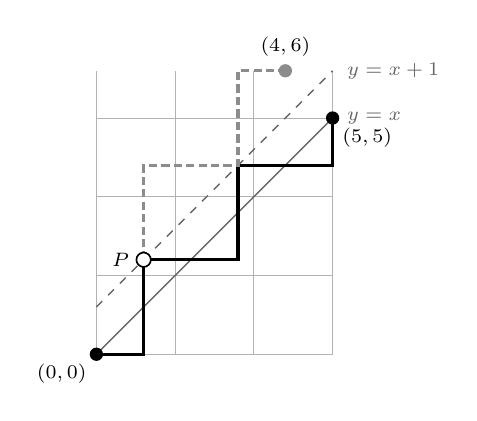
\begin{tikzpicture}[font=\scriptsize, x=0.6cm, y=0.6cm]
\draw[black!30, line width=0.3pt] (0,0) grid (5,6);
\draw[black!60, line width=0.5pt] (0,0) -- (5,5);
\draw[black!60, line width=0.5pt, dashed] (0,1) -- (5,6);
\node[anchor=west, black!60] at (5.1,5) {$y=x$};
\node[anchor=west, black!60] at (5.1,6) {$y=x+1$};
\draw[line width=1.2pt] (0,0) -- (1,0) -- (1,2) -- (3,2) -- (3,4) -- (5,4) -- (5,5);
\draw[line width=1.2pt, black!45, dash pattern=on 3pt off 1.5pt] (1,2) -- (1,4) -- (3,4) -- (3,6) -- (4,6);
\fill (0,0) circle (2.4pt); \fill (5,5) circle (2.4pt);
\fill[black!45] (4,6) circle (2.4pt);
\draw[fill=white, line width=0.6pt] (1,2) circle (2.6pt);
\node[anchor=north east] at (0,0) {$(0,0)$};
\node[anchor=north west] at (5,5) {$(5,5)$};
\node[anchor=south] at (4,6.1) {$(4,6)$};
\node[anchor=east] at (0.9,2) {$P$};
\end{tikzpicture}}{The reflection principle for $n=5$. The bad path $RUURRUURRU$ (black) from $(0,0)$ to $(5,5)$ first reaches the line $y=x+1$ at $P=(1,2)$. Reflecting its part after $P$ in that line (grey, dashed) gives a path from $(0,0)$ to $(4,6)$. Every path to $(4,6)$ arises in this way from exactly one bad path.\label{fig:reflection}}
\end{figure}

Catalan numbers count a wide variety of objects; Stanley's monograph lists more than two hundred~\cite{stanley2015catalan}. A product $x_0x_1\cdots x_n$ of $n+1$ factors can be computed in $C_n$ different orders, by the recurrence: the last multiplication combines a product of the first $k+1$ factors with a product of the remaining $n-k$, and each part can be computed in $C_k$ and $C_{n-k}$ ways. For matrices, the different orders give the same result but can differ enormously in cost, and Volume~IV shows how to find the cheapest by dynamic programming. The binary trees with $n$ nodes are also counted by $C_n$, as \cref{sec:trees} explains. By \cref{prop:binomial-size} and Stirling's formula, $C_n$ grows roughly like $4^n/n^{3/2}$.

\subsection{Evaluating Sums}

Counting problems often lead to sums, and a few techniques evaluate a large share of them. We describe three: telescoping, the calculus of falling factorials and the exchange of the order of summation~\cite[Chap.~2]{graham1994concrete}.

\begin{proposition}[Telescoping]
\label{prop:telescoping}
For every sequence $(a_k)$ of complex numbers and all integers $m\le n+1$,
\[
\sum_{k=m}^{n}(a_{k+1}-a_k)=a_{n+1}-a_m .
\]
\end{proposition}

\begin{proof}
By induction on $n$, starting at $n=m-1$, where both sides are $0$. If the identity holds for $n$, adding $a_{n+2}-a_{n+1}$ to both sides gives it for $n+1$.
\end{proof}

The art lies in recognising a term as a difference. Since $\frac1{k(k+1)}=\frac1k-\frac1{k+1}$ and $k\cdot k!=(k+1)!-k!$,
\[
\sum_{k=1}^{n}\frac1{k(k+1)}=1-\frac1{n+1},\qquad\sum_{k=1}^{n}k\cdot k!=(n+1)!-1 .
\]
Pascal's rule says that $\binom{j}{k}=\binom{j+1}{k+1}-\binom{j}{k+1}$, and telescoping then gives a second proof of the hockey stick identity.

Differences of falling factorials behave like derivatives of powers. For $m\ge1$,
\begin{equation}
(x+1)^{\underline m}-x^{\underline m}=(x+1)\,x^{\underline{m-1}}-x^{\underline{m-1}}\,(x-m+1)=m\,x^{\underline{m-1}},
\label{eq:falling-difference}
\end{equation}
which is the discrete analogue of $(x^m)'=mx^{m-1}$. Telescoping \eqref{eq:falling-difference} with $m+1$ in place of $m$ over $x=0,1,\ldots,n-1$ gives
\begin{equation}
\sum_{k=0}^{n-1}k^{\underline m}=\frac{n^{\underline{m+1}}}{m+1},
\label{eq:falling-sum}
\end{equation}
the discrete analogue of $\int_0^nx^m\,dx=n^{m+1}/(m+1)$. Dividing by $m!$ turns \eqref{eq:falling-sum} into the hockey stick identity once more. To sum ordinary powers, one expresses them through falling factorials, for example $k^2=k^{\underline2}+k^{\underline1}$, and sums term by term: $\sum_{k=0}^{n-1}k^2=n^{\underline3}/3+n^{\underline2}/2$. Graham, Knuth and Patashnik develop this \term{finite calculus} systematically~\cite[Sect.~2.6]{graham1994concrete}.

A double sum over a triangle of indices can be added row by row or column by column:
\begin{equation}
\sum_{k=1}^{n}\sum_{j=1}^{k}a_{j,k}=\sum_{j=1}^{n}\sum_{k=j}^{n}a_{j,k} .
\label{eq:exchange}
\end{equation}
Both sides add the numbers $a_{j,k}$ over the same finite set of index pairs $\{(j,k): 1\le j\le k\le n\}$, grouped in two different ways, and the general associative and commutative laws of addition, which follow from those for two terms by induction, say that the grouping does not matter. Exchanging the order often turns an awkward inner sum into a simple one. The \term{harmonic numbers}
\[
H_n\coloneqq\sum_{k=1}^{n}\frac1k=1+\frac12+\cdots+\frac1n
\]
provide an example. They begin $H_1=1$, $H_2=\frac32$, $H_3=\frac{11}6$, $H_4=\frac{25}{12}$, and $H_{10}=\frac{7381}{2520}\approx2.929$. With $a_{j,k}=1/j$, \eqref{eq:exchange} gives
\[
\sum_{k=1}^{n}H_k=\sum_{k=1}^{n}\sum_{j=1}^{k}\frac1j=\sum_{j=1}^{n}\frac{n-j+1}{j}=(n+1)H_n-n .
\]
Harmonic numbers occur constantly in the analysis of algorithms: if quicksort spends $m-1$ comparisons on partitioning a list of $m$ keys, its average number of comparisons on $n$ distinct keys is $2(n+1)H_n-4n$ (Volume~IV), and the average number of divisors in \eqref{eq:divisor-sum} is at most $H_N$. \Cref{ch:series} shows that $H_n$ differs from $\ln n$ by a quantity that tends to a constant, so that $H_n$ grows without bound, but very slowly.

\section{Generating Functions}
\label{sec:gf}

A sequence $a_0,a_1,a_2,\ldots$ of numbers is an infinite object, and a recurrence describes it one term at a time. A generating function packs the whole sequence into a single object, the power series $\sum_na_nx^n$, so that operations on sequences become algebraic operations on series. Multiplying two series, for instance, combines the counts in exactly the way the sum and product rules do. The idea goes back to the eighteenth century, to de Moivre's treatment of recurrent sequences~\cite[Sect.~1.2.8]{knuth1997taocp1} and Euler's work on partitions~\cite{andrews1976partitions}, and it turns many counting problems into problems of algebra~\cite{wilf2006,flajolet2009}.

\subsection{Formal Power Series}

In calculus, a power series is a function of $x$, defined where the series converges (\cref{ch:series}). In counting, convergence is beside the point: the series is merely a convenient way of writing the sequence of its coefficients, and $x$ is a placeholder.

\begin{definition}[Formal power series]
\label{def:fps}
A \term{formal power series} with complex coefficients is an expression
\[
A(x)=\sum_{n\ge0}a_nx^n=a_0+a_1x+a_2x^2+\cdots
\]
that stands for the sequence $(a_0,a_1,a_2,\ldots)$ of its \term{coefficients}; the symbol $x$ is not a number. We write $[x^n]A(x)\coloneqq a_n$ for the coefficient of $x^n$. Two series are equal if all their coefficients agree. The sum and the product of $A(x)=\sum a_nx^n$ and $B(x)=\sum b_nx^n$ are defined by
\[
A(x)+B(x)\coloneqq\sum_{n\ge0}(a_n+b_n)x^n,\qquad A(x)B(x)\coloneqq\sum_{n\ge0}\Bigl(\sum_{k=0}^{n}a_kb_{n-k}\Bigr)x^n .
\]
The set of formal power series is denoted $\mathbb C[[x]]$. The \term{generating function} of a sequence $(a_n)$ is the formal power series $\sum_na_nx^n$.
\end{definition}

The product is the rule for multiplying polynomials, applied to infinite series: the coefficient of $x^n$ collects the products $a_kx^k\cdot b_{n-k}x^{n-k}$. Each coefficient of the product is a finite sum, which is why no convergence is needed. The sequence of these coefficients is called the \term{convolution} of $(a_n)$ and $(b_n)$; it reappears in the discrete Fourier transform of Volume~XI. A polynomial is a series with only finitely many nonzero coefficients, and a number $c$ is identified with the series $c+0x+0x^2+\cdots$. The series $1+x+x^2+\cdots$, all of whose coefficients are $1$, is a perfectly good formal power series, and so is $\sum_nn!\,x^n$, although as a function the latter converges only at $x=0$.

\begin{proposition}
\label{prop:fps-ring}
\leavevmode
\begin{enumerate}
\item $\mathbb C[[x]]$ is a commutative ring, with zero element $0$ and unit element $1$.
\item A series $A(x)$ has an inverse in $\mathbb C[[x]]$, that is, a series $B(x)$ with $A(x)B(x)=1$, if and only if $a_0\ne0$.
\item If $A(x)B(x)=0$, then $A(x)=0$ or $B(x)=0$.
\end{enumerate}
\end{proposition}

\begin{proof}
(i) The axioms for addition hold coefficientwise, and the commutativity of multiplication and the distributive law follow directly from the definition. For associativity, both $[x^n]\bigl(A(x)B(x)\bigr)C(x)$ and $[x^n]A(x)\bigl(B(x)C(x)\bigr)$ are equal to the sum of $a_ib_jc_k$ over all triples $(i,j,k)\in\mathbb N^3$ with $i+j+k=n$.

(ii) The equation $A(x)B(x)=1$ means $a_0b_0=1$ and $\sum_{k=0}^{n}a_kb_{n-k}=0$ for $n\ge1$. If $a_0=0$, the first equation has no solution. If $a_0\ne0$, the equations are solved recursively by
\[
b_0=\frac1{a_0},\qquad b_n=-\frac1{a_0}\sum_{k=1}^{n}a_kb_{n-k}\quad(n\ge1),
\]
since each $b_n$ is determined by $b_0,\ldots,b_{n-1}$.

(iii) If $A$ and $B$ are both nonzero, let $a_i$ and $b_j$ be their first nonzero coefficients. Then $[x^{i+j}]A(x)B(x)=a_ib_j\ne0$, because all other products in this coefficient involve some $a_k$ with $k<i$ or some $b_l$ with $l<j$.
\end{proof}

The inverse of $A(x)$ is written $1/A(x)$. The most important example is the geometric series. Since $(1-x)(1+x+x^2+\cdots)=1$, all coefficients of $x^n$ with $n\ge1$ cancelling in pairs,
\begin{equation}
\frac1{1-x}=\sum_{n\ge0}x^n,\qquad\text{and more generally}\qquad\frac1{1-cx}=\sum_{n\ge0}c^nx^n\quad(c\in\mathbb C).
\label{eq:geometric-series}
\end{equation}
These are identities in $\mathbb C[[x]]$, valid without any condition on $x$, which is not a number. When $|x|<1$ is a number, the series also converges to $1/(1-x)$ in the sense of calculus, and \cref{ch:series} shows that formal and analytic computations agree wherever the series converge; but the formal theory does not need this.

\begin{proposition}
\label{prop:gf-rules}
Let $A(x)=\sum a_nx^n$ and $m\in\mathbb N$.
\begin{enumerate}
\item $x^mA(x)=\sum_{n\ge m}a_{n-m}x^n$ (shift).
\item $\dfrac{A(x)}{1-x}=\sum_{n\ge0}(a_0+a_1+\cdots+a_n)x^n$ (partial sums).
\item $\dfrac1{(1-x)^k}=\sum_{n\ge0}\dbinom{n+k-1}{k-1}x^n$ for every $k\ge1$.
\item If $a_n$ counts the objects of size $n$ in a class $\mathcal A$ and $b_n$ the objects of size $n$ in a class $\mathcal B$, then $[x^n]A(x)B(x)$ counts the pairs $(\alpha,\beta)$ with $\alpha\in\mathcal A$, $\beta\in\mathcal B$ and total size $n$.
\end{enumerate}
\end{proposition}

\begin{proof}
(i) is immediate from the definition of the product, and (ii) is the product with $\sum x^n$, whose coefficients are all $1$. For (iv), sort the pairs of total size $n$ by the size $k$ of $\alpha$: by the product rule there are $a_kb_{n-k}$ pairs with $|\alpha|=k$, and by the sum rule $\sum_ka_kb_{n-k}$ pairs in all. By induction, the coefficient of $x^n$ in a product of $k$ series is the sum of the products $a^{(1)}_{j_1}\cdots a^{(k)}_{j_k}$ over all $(j_1,\ldots,j_k)\in\mathbb N^k$ with $j_1+\cdots+j_k=n$. For (iii), all coefficients of the $k$ factors $1/(1-x)=\sum x^j$ are $1$, so $[x^n](1-x)^{-k}$ is the number of solutions of $j_1+\cdots+j_k=n$ in natural numbers, which is $\binom{n+k-1}{k-1}$ by \cref{thm:multisets}.
\end{proof}

Part (iv) explains the usefulness of generating functions for counting. Suppose, for instance, that we want the number of ways to pay $n$ units with coins of $1$ and $2$ units. A payment consists of some coins of $1$ unit, counted by $1/(1-x)=1+x+x^2+\cdots$ (one way to make each amount), and some coins of $2$ units, counted by $1/(1-x^2)=1+x^2+x^4+\cdots$. By (iv), the number of payments of $n$ units is $[x^n]\,1/\bigl((1-x)(1-x^2)\bigr)$, which by (ii) is the number of even numbers among $0,\ldots,n$, namely $\lfloor n/2\rfloor+1$. With more coin values the same reasoning leads to products with more factors, and in the limit to the partitions treated below.

\subsection{Solving Recurrences}

Let $F(x)=\sum_nF_nx^n$ be the generating function of the Fibonacci numbers. The recurrence $F_n=F_{n-1}+F_{n-2}$ for $n\ge2$, with $F_0=0$ and $F_1=1$, says that the series $F(x)-xF(x)-x^2F(x)$ has the coefficients $F_0=0$ for $n=0$, $F_1-F_0=1$ for $n=1$, and $F_n-F_{n-1}-F_{n-2}=0$ for $n\ge2$, by the shift rule. Hence $(1-x-x^2)F(x)=x$, and since $1-x-x^2$ has constant term $1$, it is invertible:
\[
F(x)=\frac{x}{1-x-x^2}.
\]
The denominator factors as $1-x-x^2=(1-\phi x)(1-\hat\phi x)$, because $\phi+\hat\phi=1$ and $\phi\hat\phi=-1$. Splitting into partial fractions,
\[
\frac{x}{(1-\phi x)(1-\hat\phi x)}=\frac1{\sqrt5}\Bigl(\frac1{1-\phi x}-\frac1{1-\hat\phi x}\Bigr),
\]
as one checks by bringing the right side to a common denominator and using $\phi-\hat\phi=\sqrt5$. By \eqref{eq:geometric-series}, the coefficient of $x^n$ on the right is $(\phi^n-\hat\phi^n)/\sqrt5$, which is Binet's formula \eqref{eq:binet} again, now derived without guessing the form of the solution. The same method applies to every linear recurrence with constant coefficients: the generating function of a solution is a rational function, a quotient of two polynomials, and partial fractions give the formula of \cref{prop:linear-recurrence-k}~\cite[Sect.~7.3]{graham1994concrete}.

Generating functions also handle nonlinear recurrences. The Catalan recurrence of \cref{prop:catalan-recurrence} says that $C_{n+1}$ is the coefficient of $x^n$ in $C(x)^2$, where $C(x)\coloneqq\sum_nC_nx^n$. Multiplying by $x$ and adding $C_0=1$ gives the quadratic equation
\begin{equation}
C(x)=1+x\,C(x)^2 .
\label{eq:catalan-gf}
\end{equation}
Solving it requires square roots of power series, which come from a generalisation of the binomial theorem due to Newton~\cite[Sects.~5.1 and~5.4]{graham1994concrete}.

\begin{theorem}[Newton's binomial series]
\label{thm:newton}
For a real number $r$ let
\[
N_r(x)\coloneqq\sum_{k\ge0}\binom rkx^k ,
\]
with the binomial coefficients of \cref{def:binomial-general}. Then $N_r(x)N_s(x)=N_{r+s}(x)$ for all real $r$ and $s$, and $N_n(x)=(1+x)^n$ for $n\in\mathbb N$. In particular $N_{1/2}(x)^2=1+x$, and $N_{-n}(x)$ is the inverse of $(1+x)^n$.
\end{theorem}

\begin{proof}
The coefficient of $x^n$ in $N_r(x)N_s(x)=N_{r+s}(x)$ is the identity
\[
\sum_{k=0}^{n}\binom rk\binom s{n-k}=\binom{r+s}{n}.
\]
Fix $n$ and a natural number $s$. Both sides are polynomials in $r$, since $\binom rk=r^{\underline k}/k!$ is a polynomial in $r$ of degree $k$, and by Vandermonde's identity (\cref{thm:vandermonde}) they agree for every $r\in\mathbb N$. Their difference is therefore a polynomial with infinitely many roots, which must be the zero polynomial by \cref{cor:factor}\,(ii); so the identity holds for every real $r$ and every natural $s$. Now fix a real $r$. Both sides are polynomials in $s$ that agree for every $s\in\mathbb N$, so the same argument shows that they agree for every real $s$. For $n\in\mathbb N$, $\binom nk=0$ for $k>n$, and $N_n(x)=(1+x)^n$ is the binomial theorem. Finally $N_{1/2}^2=N_1=1+x$ and $N_{-n}N_n=N_0=1$.
\end{proof}

For a negative integer the theorem gives back \cref{prop:gf-rules}\,(iii): by \eqref{eq:upper-negation}, $[x^n]N_{-k}(-x)=(-1)^n\binom{-k}{n}=\binom{n+k-1}{n}$, the coefficient of $x^n$ in $1/(1-x)^k$. For $r=\frac12$ it provides a square root of $1+x$, and replacing $x$ by $cx$, which multiplies the coefficient of $x^n$ by $c^n$ in every series and therefore respects products, a square root $N_{1/2}(cx)$ of $1+cx$. We can now solve \eqref{eq:catalan-gf}. By \eqref{eq:catalan-gf},
\[
\bigl(1-2xC(x)\bigr)^2=1-4xC(x)+4x^2C(x)^2=1-4x\bigl(C(x)-xC(x)^2\bigr)=1-4x .
\]
So $1-2xC(x)$ and $N_{1/2}(-4x)$ are two square roots of $1-4x$ with constant term $1$. They are equal: if $S^2=T^2$, then $(S-T)(S+T)=0$, and $S+T$ has constant term $2$, so it is invertible and $S-T=0$. Comparing the coefficients of $x^{n+1}$ in $1-2xC(x)=N_{1/2}(-4x)$ gives
\[
-2C_n=\binom{1/2}{n+1}(-4)^{n+1}.
\]
The binomial coefficient is
\[
\binom{1/2}{n+1}=\frac{\frac12\bigl(-\frac12\bigr)\bigl(-\frac32\bigr)\cdots\bigl(\frac12-n\bigr)}{(n+1)!}=\frac{(-1)^n\cdot1\cdot3\cdots(2n-1)}{2^{n+1}(n+1)!}=\frac{(-1)^n(2n)!}{2^{2n+1}\,n!\,(n+1)!},
\]
where we used $1\cdot3\cdots(2n-1)=(2n)!/(2\cdot4\cdots2n)=(2n)!/(2^nn!)$. Multiplying by $(-4)^{n+1}=(-1)^{n+1}2^{2n+2}$ gives $-2(2n)!/(n!\,(n+1)!)$, and therefore
\[
C_n=\frac{(2n)!}{n!\,(n+1)!}=\frac1{n+1}\binom{2n}{n},
\]
in agreement with \cref{thm:catalan}. The two proofs are instructive in different ways: the reflection argument explains the formula, while the generating function finds it without needing a clever idea.

\subsection{Partitions}

A \term{partition} of a natural number $n$ is a way of writing $n$ as a sum of positive integers, the order of the summands being irrelevant. The number of partitions of $n$ is denoted $p(n)$, with $p(0)=1$. For example, $p(5)=7$:
\[
5=4+1=3+2=3+1+1=2+2+1=2+1+1+1=1+1+1+1+1 .
\]
A partition is specified by the number $j_k\in\mathbb N$ of summands equal to $k$, for each $k\ge1$, subject to $\sum_kk\,j_k=n$. The summands equal to $k$ contribute $kj_k$ to the total, and the generating function for this contribution is $1+x^k+x^{2k}+\cdots=1/(1-x^k)$. By \cref{prop:gf-rules}\,(iv), the number of partitions of $n$ into summands at most $N$ is the coefficient of $x^n$ in
\[
P_N(x)\coloneqq\prod_{k=1}^{N}\frac1{1-x^k}.
\]
For $N\ge n$ no summand can exceed $N$, so $[x^n]P_N(x)=p(n)$ for every $N\ge n$. In this sense,
\[
\sum_{n\ge0}p(n)x^n=\prod_{k\ge1}\frac1{1-x^k},
\]
the infinite product being defined coefficientwise: the coefficient of $x^n$ is the common value of $[x^n]P_N(x)$ for all $N\ge n$. This formula is due to Euler~\cite{andrews1976partitions}. The sequence begins
\[
1,\ 1,\ 2,\ 3,\ 5,\ 7,\ 11,\ 15,\ 22,\ 30,\ 42\qquad(n=0,\ldots,10),
\]
and grows faster than any power of $n$ but slower than any exponential $c^n$ with $c>1$: $p(100)=190\,569\,292$. In 1918 Hardy and Ramanujan found the asymptotic formula $p(n)\approx e^{\pi\sqrt{2n/3}}/(4n\sqrt3)$, which exceeds the true value at $n=100$ by less than five per cent, together with a much more precise asymptotic series, accurate enough to determine $p(n)$ exactly~\cite{hardyramanujan1918}. Partitions of a different kind, partitions of a \emph{set} into blocks, were counted by the Bell numbers in \cref{sec:ie-pigeonhole}.

\subsection{The Distribution of a Rank Sum}

Generating functions are not only a theoretical device; they compute. Statistics provides a typical example. Suppose $n$ measured differences, for instance between a patient's blood pressure before and after a treatment, are ranked by their absolute value from $1$ (smallest) to $n$ (largest), and let $T$ be the sum of the ranks of the positive differences. If the treatment has no effect, each difference is as likely to be positive as negative, independently of the others, and each of the $2^n$ sets of ``positive'' ranks is equally likely. To judge whether an observed $T$ is unusually small or large, we need the number $c_n(s)$ of subsets of $\{1,\ldots,n\}$ whose elements add up to $s$. This is the null distribution of Wilcoxon's signed-rank statistic~\cite{wilcoxon1945}.

By the reasoning of the combinatorial proof of \cref{thm:binomial}, expanding the product $\prod_{i=1}^{n}(1+q^i)$ means choosing either $1$ or $q^i$ from each factor, that is, choosing a subset $S\subseteq\{1,\ldots,n\}$, and the choice produces the term $q^{\sum_{i\in S}i}$. Hence
\[
\sum_{s\ge0}c_n(s)\,q^s=\prod_{i=1}^{n}(1+q^i).
\]
Multiplying out the product one factor at a time is an efficient algorithm, \cref{alg:subset-sums}. Multiplication by $1+q^i$ adds to each coefficient the coefficient $i$ places lower: $c_i(s)=c_{i-1}(s)+c_{i-1}(s-i)$, which is also clear combinatorially, since a subset of $\{1,\ldots,i\}$ with sum $s$ either omits $i$ or consists of $i$ and a subset of $\{1,\ldots,i-1\}$ with sum $s-i$. Running $s$ downwards lets the algorithm overwrite a single array, because $c(s-i)$ is read before it is updated.

\begin{algorithm}
\begin{algorithmic}[1]
\Require a natural number $n$
\Ensure $c[0..N]$ with $N=n(n+1)/2$, where $c[s]$ is the number of subsets of $\{1,\ldots,n\}$ with sum $s$
\Name{SubsetSumCounts}{n}
\State $N\gets n(n+1)/2$; \ $c[0]\gets1$; \ $c[s]\gets0$ for $s=1,\ldots,N$
\For{$i\gets1$ \textbf{to} $n$} \Comment{multiply by $1+q^i$}
  \For{$s\gets i(i+1)/2$ \textbf{down to} $i$} \Comment{$i(i+1)/2$ is the largest sum so far}
    \State $c[s]\gets c[s]+c[s-i]$
  \EndFor
\EndFor
\State \Return $c$
\end{algorithmic}
\caption{The coefficients of $\prod_{i=1}^{n}(1+q^i)$. After the pass for $i$, $c[s]$ is the number of subsets of $\{1,\ldots,i\}$ with sum $s$. The algorithm performs $n+\binom{n+1}{3}\approx n^3/6$ additions.}
\label{alg:subset-sums}
\end{algorithm}

For $n=10$ there are $2^{10}=1024$ subsets and the sums range from $0$ to $55$. \Cref{fig:rank-sum} shows the counts. The distribution is symmetric about $27.5$, because taking complements sends a subset with sum $s$ to one with sum $55-s$. Only $25$ of the $1024$ subsets have a sum of at most $8$, so an observed $T\le8$ would occur with probability $25/1024\approx0.024$ if the treatment had no effect; such probabilities are the $p$-values of Volume~XIV, where exact null distributions of many rank statistics are computed by counting of this kind. The two-sample rank-sum statistic of Wilcoxon, Mann and Whitney leads in the same way to the number of $k$-element subsets of $\{1,\ldots,n\}$ with a given sum~\cite{mannwhitney1947}.

\begin{figure}
\sdfloat{%
\begin{tikzpicture}
\begin{axis}[sdplot, width=0.72\textwidth, height=0.38\textwidth, ybar, bar width=1.9pt,
  xmin=-1.5, xmax=56.5, ymin=0, ymax=44, xtick={0,10,20,30,40,50}, ytick={0,10,20,30,40},
  xlabel={sum $s$}, ylabel={$c_{10}(s)$}]
\addplot[fill=sdfill, draw=black, line width=0.3pt] coordinates {(0,1) (1,1) (2,1) (3,2) (4,2) (5,3) (6,4) (7,5) (8,6) (9,8) (10,10) (11,11) (12,13) (13,15) (14,17) (15,20) (16,22) (17,24) (18,27) (19,29) (20,31) (21,33) (22,35) (23,36) (24,38) (25,39) (26,39) (27,40) (28,40) (29,39) (30,39) (31,38) (32,36) (33,35) (34,33) (35,31) (36,29) (37,27) (38,24) (39,22) (40,20) (41,17) (42,15) (43,13) (44,11) (45,10) (46,8) (47,6) (48,5) (49,4) (50,3) (51,2) (52,2) (53,1) (54,1) (55,1)};
\end{axis}
\end{tikzpicture}}{The number $c_{10}(s)$ of subsets of $\{1,\ldots,10\}$ with sum $s$, the coefficients of $\prod_{i=1}^{10}(1+q^i)$. The $1024$ subsets are distributed symmetrically about $27.5$, and the largest counts, $40$, occur at $s=27$ and $s=28$.\label{fig:rank-sum}}
\end{figure}

\section{Graphs}
\label{sec:graphs}

In 1736 Leonhard Euler considered the seven bridges of K\"onigsberg and asked whether a walk through the town could cross each bridge exactly once. He observed that only the pattern of connections matters, not the shapes or distances, and he answered the question by counting, at each piece of land, the bridges that end there~\cite{euler1741konigsberg,biggs1976}. A structure consisting of objects and connections between pairs of them is a graph. Graphs describe road and computer networks, molecules, the dependencies between the tasks of a project and the steps of a computation. In this series they appear as the data of the algorithms of Volume~IV and as the pattern of nonzero entries of a sparse matrix in Volume~IX. This section introduces the basic vocabulary and proves the first theorems.

\subsection{Definitions and Examples}

\begin{definition}[Graph]
\label{def:graph}
A \term{graph} $G=(V,E)$ consists of a finite nonempty set $V$, whose elements are the \term{vertices} of $G$, and a set $E\subseteq\binom V2$ of $2$-element subsets of $V$, the \term{edges} of $G$. An edge $\{u,v\}$ is also written $uv$ (or $vu$). If $uv\in E$, the vertices $u$ and $v$ are \term{adjacent}, or \term{neighbours}, and they are the \term{endpoints} of the edge, which is \term{incident} with them. The \term{degree} $\deg(v)$ of a vertex $v$ is the number of its neighbours.
\end{definition}

Graphs are drawn with a dot for each vertex and a line for each edge, as in \cref{fig:graph-examples}; where the dots are placed and how the lines are drawn carries no meaning. The definition excludes edges from a vertex to itself (\term{loops}) and several edges between the same two vertices (\term{multiple edges}). Graphs in this sense are often called \term{simple graphs}, and graphs that allow loops and multiple edges are called \term{multigraphs}; Euler's bridges form a multigraph, since some pieces of land are joined by two bridges. A graph with $n$ vertices has at most $\binom n2$ edges. On a fixed set of $n$ vertices, every subset of the $\binom n2$ possible edges gives a graph, so by \cref{prop:power-set-size} there are
\[
2^{\binom n2}
\]
graphs with vertex set $\{1,\ldots,n\}$: $8$ for $n=3$, $64$ for $n=4$, $1024$ for $n=5$ and about $3.5\times10^{13}$ for $n=10$.

Some graphs occur so often that they have names.
\begin{itemize}
\item The \term{complete graph} $K_n$ has $n$ vertices and all $\binom n2$ possible edges.
\item The \term{complete bipartite graph} $K_{m,n}$ has as vertex set the union of disjoint sets $X$ and $Y$ with $m$ and $n$ elements, and as edges all $mn$ pairs $xy$ with $x\in X$ and $y\in Y$.
\item The \term{cycle} of length $n\ge3$ has vertex set $\mathbb Z/n\mathbb Z$ and the $n$ edges $\{[i],[i+1]\}$; it is drawn as a polygon. The \term{path} with $n$ vertices has vertex set $\{1,\ldots,n\}$ and the $n-1$ edges $\{i,i+1\}$.
\item The \term{hypercube} $Q_d$ has as vertices the $2^d$ binary words of length $d$, two words being adjacent if they differ in exactly one position. Hypercubes describe the interconnection of some parallel computers, and a path through all vertices of $Q_d$ is a Gray code, a listing of all binary words in which successive words differ in one bit~\cite[Sect.~7.2.1.1]{knuth2011taocp4a}.
\end{itemize}

\begin{figure}
\tikzset{gv/.style={circle, fill=black, inner sep=0pt, minimum size=4pt},
  ge/.style={line width=0.5pt}}
\sdpanel{A}{\begin{tikzpicture}[font=\scriptsize]
\foreach \i in {0,...,4} {\node[gv] (a\i) at ({90+72*\i}:1) {};}
\foreach \i in {0,...,4} {\foreach \j in {0,...,4} {\ifnum\i<\j \draw[ge] (a\i) -- (a\j); \fi}}
\path (0,-1.25) -- (0,1.25);
\end{tikzpicture}}\hfill
\sdpanel{B}{\begin{tikzpicture}[font=\scriptsize]
\foreach \i in {0,1,2} {\node[gv] (x\i) at (\i*0.9,1.6) {}; \node[gv] (y\i) at (\i*0.9,0) {};}
\foreach \i in {0,1,2} {\foreach \j in {0,1,2} {\draw[ge] (x\i) -- (y\j);}}
\node[above=1pt] at (x1) {$X$}; \node[below=1pt] at (y1) {$Y$};
\path (0,-0.45) -- (0,2.05);
\end{tikzpicture}}\hfill
\sdpanel{C}{\begin{tikzpicture}[font=\scriptsize]
\foreach \w/\x/\y in {000/0/0,100/1.3/0,010/0/1.3,110/1.3/1.3,001/0.55/0.5,101/1.85/0.5,011/0.55/1.8,111/1.85/1.8}
  {\node[gv] (q\w) at (\x,\y) {};}
\foreach \a/\b in {000/100,000/010,000/001,100/110,100/101,010/110,010/011,001/101,001/011,110/111,101/111,011/111}
  {\draw[ge] (q\a) -- (q\b);}
\node[below left=0pt] at (q000) {$000$}; \node[below=1pt] at (q100) {$100$};
\node[left=1pt] at (q010) {$010$}; \node[above right=0pt] at (q111) {$111$};
\node[right=1pt] at (q101) {$101$}; \node[above=1pt] at (q011) {$011$};
\node[below left=-1pt] at (q110) {$110$}; \node[above right=-1pt] at (q001) {$001$};
\path (0,-0.45) -- (0,2.05);
\end{tikzpicture}}\hfill
\sdpanel{D}{\begin{tikzpicture}[font=\scriptsize]
\node[gv] (d1) at (0,0) {}; \node[gv] (d2) at (1,0) {}; \node[gv] (d3) at (0.5,0.85) {}; \node[gv] (d4) at (0.5,1.75) {};
\node[gv] (d5) at (1.7,1.0) {}; \node[gv] (d6) at (2.3,1.75) {}; \node[gv] (d7) at (2.3,0.3) {};
\draw[ge] (d1) -- (d2) -- (d3) -- (d1); \draw[ge] (d3) -- (d4);
\draw[ge] (d5) -- (d6); \draw[ge] (d5) -- (d7);
\foreach \v/\dg/\p in {d1/2/below,d2/2/below,d3/3/left,d4/1/left,d5/2/left,d6/1/right,d7/1/right} {\node[\p=1pt] at (\v) {$\dg$};}
\path (0,-0.45) -- (0,2.05);
\end{tikzpicture}}
\caption{Examples of graphs. (A) The complete graph $K_5$, with $10$ edges. (B) The complete bipartite graph $K_{3,3}$, with $9$ edges. (C) The hypercube $Q_3$, with $8$ vertices and $12$ edges; two words are adjacent when they differ in one bit. (D) A graph with $7$ vertices, $6$ edges and two components; each vertex is labelled with its degree, and the degrees add up to $12=2\cdot6$.}
\label{fig:graph-examples}
\end{figure}

Two graphs that differ only in the names of their vertices are regarded as having the same structure. Graphs $G=(V,E)$ and $G'=(V',E')$ are \term{isomorphic} if there is a bijection $f\colon V\to V'$ such that $uv\in E$ if and only if $f(u)f(v)\in E'$, for all $u,v\in V$; the bijection is an \term{isomorphism}. The $8$ graphs with vertex set $\{1,2,3\}$ fall into $4$ classes of isomorphic graphs, distinguished by their number of edges, and the $64$ graphs on $\{1,2,3,4\}$ fall into $11$ classes. Counting graphs up to isomorphism is considerably harder than counting graphs on a fixed vertex set, because the classes have different sizes~\cite{harary1973enumeration}.

The degrees of a graph are not independent of one another. The following lemma already appears, in the language of bridges and pieces of land, in Euler's paper~\cite{euler1741konigsberg,biggs1976}. It is often called the first theorem of graph theory, and it is an instance of double counting.

\begin{lemma}[Handshake lemma]
\label{lem:handshake}
For every graph $G=(V,E)$,
\[
\sum_{v\in V}\deg(v)=2|E| .
\]
Consequently, the number of vertices of odd degree is even.
\end{lemma}

\begin{proof}
Count the pairs $(v,e)$ with $v\in V$, $e\in E$ and $v\in e$ in two ways (\cref{prop:double-counting}). For a fixed vertex $v$ there are $\deg(v)$ such pairs, one for each incident edge; for a fixed edge $e$ there are $2$, one for each endpoint. Hence $\sum_v\deg(v)=2|E|$. The vertices of even degree contribute an even number to this sum, so the vertices of odd degree must contribute an even number too, which requires an even number of them.
\end{proof}

The name comes from the interpretation in which the vertices are the guests at a party and the edges are the handshakes between them: the total number of hands shaken is twice the number of handshakes, and the number of guests who shook an odd number of hands is even. In $K_n$ every degree is $n-1$, and the lemma gives $n(n-1)=2\binom n2$. In $Q_d$ every vertex has $d$ neighbours, obtained by changing one of its $d$ bits, so $Q_d$ has $d\,2^d/2=d\,2^{d-1}$ edges, $12$ for $d=3$. There is no graph with five vertices all of degree $3$, since the sum $15$ would be odd. A graph in which every vertex has degree $k$ is called $k$-\term{regular}.

A graph $H=(W,F)$ is a \term{subgraph} of $G=(V,E)$ if $W\subseteq V$ and $F\subseteq E$. For $W\subseteq V$ nonempty, the \term{induced subgraph} $G[W]$ has vertex set $W$ and all the edges of $G$ with both endpoints in $W$. Removing a vertex $v$ and its incident edges leaves the induced subgraph $G-v\coloneqq G[V\setminus\{v\}]$, and removing an edge $e$ leaves $G-e\coloneqq(V,E\setminus\{e\})$.

\subsection{Walks, Paths and Connectedness}

\begin{definition}[Walk, path, cycle]
\label{def:walk}
Let $G=(V,E)$ be a graph. A \term{walk} of length $k$ from $u$ to $v$ is a sequence $(v_0,v_1,\ldots,v_k)$ of vertices with $v_0=u$, $v_k=v$ and $v_{i-1}v_i\in E$ for $i=1,\ldots,k$. It is a \term{path} if its vertices are pairwise distinct, and it is \term{closed} if $k\ge1$ and $v_0=v_k$. A \term{cycle} is a closed walk of length $k\ge3$ whose vertices $v_0,\ldots,v_{k-1}$ are pairwise distinct.
\end{definition}

A walk may repeat vertices and edges, a path may not. A walk of length $0$ consists of a single vertex. In a simple graph, a closed walk of length $2$ goes along an edge and back, and it is not a cycle; this is why cycles are required to have length at least $3$. A cycle in the sense of the definition, read as a subgraph with its $k$ vertices and $k$ edges, is a copy of the cycle graph of length $k$.

\begin{lemma}
\label{lem:walk-path}
If there is a walk of length $k$ from $u$ to $v$, then there is a path from $u$ to $v$ of length at most $k$.
\end{lemma}

\begin{proof}
Among all walks from $u$ to $v$, which exist by hypothesis, choose one, $(v_0,\ldots,v_l)$, of least length; then $l\le k$. If two of its vertices coincided, $v_i=v_j$ with $i<j$, then deleting $v_{i+1},\ldots,v_j$ would give the shorter walk $(v_0,\ldots,v_i,v_{j+1},\ldots,v_l)$ from $u$ to $v$, contradicting the choice. Hence the walk is a path.
\end{proof}

\begin{proposition}
\label{prop:components}
For vertices $u$ and $v$ of a graph $G$, write $u\approx v$ if there is a walk from $u$ to $v$. This is an equivalence relation on $V$.
\end{proposition}

\begin{proof}
It is reflexive, by the walk $(u)$ of length $0$; symmetric, because a walk can be reversed; and transitive, because a walk from $u$ to $v$ followed by a walk from $v$ to $w$ is a walk from $u$ to $w$.
\end{proof}

By \cref{thm:partition}, the equivalence classes of $\approx$ partition $V$. The subgraphs induced by the classes are the \term{connected components} of $G$, and $G$ is \term{connected} if it has a single component, that is, if any two vertices are joined by a walk, or equivalently, by \cref{lem:walk-path}, by a path. The graph of \cref{fig:graph-examples}D has two components. The \term{distance} $d(u,v)$ between vertices of the same component is the least length of a walk from $u$ to $v$, which by \cref{lem:walk-path} is the length of a shortest path. Finding the components and the distances of a graph with millions of vertices are basic tasks of graph algorithms, solved by the breadth-first and depth-first searches of Volume~IV.

\subsection{Bipartite Graphs}

\begin{definition}[Bipartite graph]
\label{def:bipartite}
A graph $G=(V,E)$ is \term{bipartite} if $V$ is the union of two disjoint sets $X$ and $Y$ such that every edge has one endpoint in $X$ and the other in $Y$.
\end{definition}

Equivalently, the vertices can be coloured with two colours so that adjacent vertices receive different colours. The graphs $K_{m,n}$ are bipartite, by definition. So is $Q_d$: changing one bit of a word changes the parity of the number of ones, so the words with an even number of ones and those with an odd number form the two sides. Bipartite graphs model relations between two kinds of objects, such as workers and the jobs they can do, or the rows and the columns of a matrix that hold nonzero entries; Volume~IX treats matchings in such graphs. A cycle of odd length is not bipartite: going around it, the colours must alternate, and after an odd number of steps the starting vertex would need the other colour. Odd cycles are in fact the only obstruction. The proof needs a lemma about closed walks.

\begin{lemma}
\label{lem:odd-walk}
Every closed walk of odd length in a graph contains a cycle of odd length, in the sense that the vertices and edges of such a cycle are among those of the walk.
\end{lemma}

\begin{proof}
We use strong induction on the length $k$ of the closed walk $(v_0,\ldots,v_k)$, $v_k=v_0$. Since the graph has no loops, $k\ne1$, so $k\ge3$. If the vertices $v_0,\ldots,v_{k-1}$ are pairwise distinct, the walk is itself a cycle of odd length. Otherwise $v_i=v_j$ for some $0\le i<j\le k-1$. The walk then splits into the two closed walks $(v_i,v_{i+1},\ldots,v_j)$ of length $j-i$ and $(v_j,v_{j+1},\ldots,v_k=v_0,v_1,\ldots,v_i)$ of length $k-(j-i)$, both of length at least $1$ and less than $k$. Their lengths add up to the odd number $k$, so one of them is odd, and by the inductive hypothesis it contains an odd cycle.
\end{proof}

\begin{theorem}[K\H{o}nig]
\label{thm:bipartite}
A graph is bipartite if and only if it contains no cycle of odd length.
\end{theorem}

\begin{proof}
Suppose $G$ is bipartite with sides $X$ and $Y$, and let $(v_0,\ldots,v_k)$ be a cycle. Consecutive vertices lie on different sides, so $v_i$ lies on the side of $v_0$ exactly when $i$ is even. Since $v_k=v_0$, $k$ is even.

Conversely, suppose $G$ has no odd cycle. It suffices to colour each component separately, so we may assume that $G$ is connected. Fix a vertex $r$ and let $X$ be the set of vertices at even distance from $r$ and $Y$ the set of vertices at odd distance. Suppose some edge $uv$ had both endpoints in $X$, or both in $Y$. Then $d(r,u)$ and $d(r,v)$ have the same parity, and a shortest path from $r$ to $u$, followed by the edge $uv$ and by a shortest path from $v$ back to $r$, is a closed walk of length $d(r,u)+1+d(r,v)$, which is odd. By \cref{lem:odd-walk}, $G$ contains an odd cycle, a contradiction. Hence every edge joins $X$ and $Y$.
\end{proof}

The theorem appears in D\'enes K\H{o}nig's book of 1936, the first book devoted to graph theory~\cite{konig1936,biggs1976}. Its proof is an algorithm: \cref{fig:bipartite} shows the layers of vertices at distance $0,1,2,\ldots$ from $r$, which breadth-first search computes, and the graph is bipartite exactly when no edge joins two vertices in layers of the same parity. If such an edge exists, the proof exhibits an odd closed walk through it, and hence an odd cycle, as a certificate that no two-colouring is possible.

\begin{figure}
\tikzset{wv/.style={circle, draw, line width=0.5pt, fill=white, inner sep=0pt, minimum size=5pt},
  bv/.style={circle, fill=black, inner sep=0pt, minimum size=5pt},
  ge/.style={line width=0.5pt}}
\sdpanel{A}{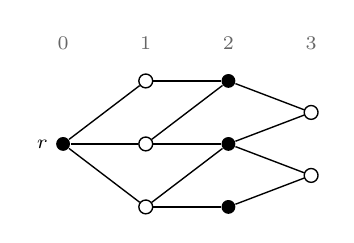
\begin{tikzpicture}[font=\scriptsize, x=1.05cm, y=0.8cm]
\foreach \l in {0,1,2,3} {\node[black!60] at (\l,2.6) {$\l$};}
\node[bv] (r) at (0,1) {}; \node[left=2pt] at (r) {$r$};
\node[wv] (a) at (1,2) {}; \node[wv] (b) at (1,1) {}; \node[wv] (c) at (1,0) {};
\node[bv] (d) at (2,2) {}; \node[bv] (e) at (2,1) {}; \node[bv] (f) at (2,0) {};
\node[wv] (g) at (3,1.5) {}; \node[wv] (h) at (3,0.5) {};
\draw[ge] (r) -- (a); \draw[ge] (r) -- (b); \draw[ge] (r) -- (c);
\draw[ge] (a) -- (d); \draw[ge] (b) -- (d); \draw[ge] (b) -- (e); \draw[ge] (c) -- (f); \draw[ge] (c) -- (e);
\draw[ge] (d) -- (g); \draw[ge] (e) -- (g); \draw[ge] (f) -- (h); \draw[ge] (e) -- (h);
\end{tikzpicture}}\hfill
\sdpanel{B}{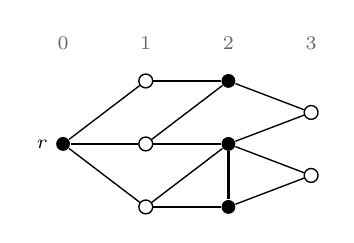
\begin{tikzpicture}[font=\scriptsize, x=1.05cm, y=0.8cm]
\foreach \l in {0,1,2,3} {\node[black!60] at (\l,2.6) {$\l$};}
\node[bv] (r) at (0,1) {}; \node[left=2pt] at (r) {$r$};
\node[wv] (a) at (1,2) {}; \node[wv] (b) at (1,1) {}; \node[wv] (c) at (1,0) {};
\node[bv] (d) at (2,2) {}; \node[bv] (e) at (2,1) {}; \node[bv] (f) at (2,0) {};
\node[wv] (g) at (3,1.5) {}; \node[wv] (h) at (3,0.5) {};
\draw[ge] (r) -- (a); \draw[ge] (r) -- (b); \draw[ge] (r) -- (c);
\draw[ge] (a) -- (d); \draw[ge] (b) -- (d); \draw[ge] (b) -- (e); \draw[ge] (c) -- (f); \draw[ge] (c) -- (e);
\draw[ge] (d) -- (g); \draw[ge] (e) -- (g); \draw[ge] (f) -- (h); \draw[ge] (e) -- (h);
\draw[line width=1.3pt] (e) -- (f);
\end{tikzpicture}}
\caption{Colouring a connected graph by the parity of the distance from a vertex $r$; the grey numbers are the distances. (A) Every edge joins a vertex at even distance (black) to a vertex at odd distance (white), so the graph is bipartite. (B) The same graph with one more edge (thick), which joins two vertices at distance $2$. The closed walk of the proof, from $r$ to one endpoint of the new edge, along it and back to $r$, has the odd length $5$; it contains an odd cycle, here the triangle formed by the new edge and the two edges that join its endpoints to their common neighbour at distance $1$.}
\label{fig:bipartite}
\end{figure}

\subsection{Directed Graphs}

In many applications the connections have a direction: a one-way street, a task that must precede another, a link from one web page to another.

\begin{definition}[Directed graph]
\label{def:digraph}
A \term{directed graph} $D=(V,A)$ consists of a finite nonempty set $V$ of vertices and a set $A\subseteq V\times V$ of \term{arcs}. The arc $(u,v)$ goes from its \term{tail} $u$ to its \term{head} $v$. The \term{out-degree} of a vertex is the number of arcs with that vertex as tail, and the \term{in-degree} the number of arcs with it as head.
\end{definition}

A directed graph is thus nothing but a relation on $V$ in the sense of \cref{def:relation}, and \cref{fig:relation}A drew one. Loops $(v,v)$ are allowed. An undirected graph can be regarded as a directed graph whose relation is symmetric and irreflexive, each edge $uv$ becoming the two arcs $(u,v)$ and $(v,u)$. By \cref{prop:double-counting}, applied to the relation $A$ itself, the out-degrees and the in-degrees both add up to $|A|$.

Directed walks, paths and cycles are defined as in \cref{def:walk}, with $(v_{i-1},v_i)\in A$ in place of $v_{i-1}v_i\in E$; here a \term{directed cycle} is a closed directed walk of length $k\ge1$ with $v_0,\ldots,v_{k-1}$ pairwise distinct, so that a loop is a directed cycle of length $1$ and two opposite arcs form one of length $2$. A vertex $v$ is \term{reachable} from $u$ if there is a directed walk from $u$ to $v$; by \cref{prop:transitive-closure}\,(iii), this is the case if $u=v$ or $u\mathrel{A^+}v$, where $A^+$ is the transitive closure of the relation $A$. Reachability is no longer symmetric, and the theory of components becomes richer than for undirected graphs (Volume~IV).

A directed graph without directed cycles is called \term{acyclic}, or a DAG (directed acyclic graph). Acyclic graphs describe precedences: an arc $(u,v)$ says that task $u$ must be completed before task $v$ can begin, and an acyclic graph is precisely one in which the tasks can be scheduled.

\begin{proposition}[Topological order]
\label{prop:topological}
The vertices of a directed graph $D=(V,A)$ with $n$ vertices can be listed as $v_1,\ldots,v_n$ in such a way that every arc goes from an earlier to a later vertex, that is, $(v_i,v_j)\in A$ implies $i<j$, if and only if $D$ is acyclic.
\end{proposition}

\begin{proof}
If such a listing exists and $(v_{i_0},v_{i_1},\ldots,v_{i_k})$ is a directed cycle, then $i_0<i_1<\cdots<i_k=i_0$, which is impossible.

Conversely, let $D$ be acyclic, and write $u\preceq v$ if $v$ is reachable from $u$. This relation is reflexive and transitive, as in \cref{prop:components}. It is antisymmetric. Suppose that $u\preceq v$ and $v\preceq u$ with $u\ne v$; then a directed walk from $u$ to $v$ followed by one from $v$ to $u$ is a closed directed walk of positive length. Among all closed directed walks of positive length in $D$ choose one, $(w_0,\ldots,w_k)$, of least length. If $w_i=w_j$ for some $0\le i<j\le k$ other than $i=0$, $j=k$, then $(w_i,\ldots,w_j)$ would be a shorter closed walk of positive length; hence $w_0,\ldots,w_{k-1}$ are distinct and the walk is a directed cycle, contrary to the assumption. So $\preceq$ is a partial order, and by \cref{thm:linear-extension} the vertices can be listed as $v_1,\ldots,v_n$ so that $v_i\prec v_j$ implies $i<j$. For an arc $(v_i,v_j)$ we have $v_i\preceq v_j$, and $v_i\ne v_j$ because a loop would be a directed cycle; so $v_i\prec v_j$ and $i<j$.
\end{proof}

Such a listing is a \term{topological order} of $D$. \Cref{fig:dag} shows an example. Build systems use topological orders to decide in which order to compile files that depend on one another, spreadsheets use them to recompute cells, and the evaluation of an arithmetic expression follows one. As the remark after \cref{thm:linear-extension} explained, the proof is an algorithm in disguise; Volume~IV gives an efficient version.

\begin{figure}
\tikzset{dv/.style={circle, draw, line width=0.5pt, inner sep=0pt, minimum size=0.46cm},
  da/.style={-{Latex[length=1.4mm]}, line width=0.5pt}}
\sdpanel{A}{\begin{tikzpicture}[font=\scriptsize]
\node[dv] (a) at (0,1.2) {$a$}; \node[dv] (b) at (0,0) {$b$};
\node[dv] (c) at (1.2,1.2) {$c$}; \node[dv] (d) at (1.2,0) {$d$};
\node[dv] (e) at (2.4,0.6) {$e$}; \node[dv] (f) at (3.6,0.6) {$f$};
\draw[da] (a) -- (c); \draw[da] (b) -- (c); \draw[da] (b) -- (d);
\draw[da] (c) -- (e); \draw[da] (d) -- (e); \draw[da] (e) -- (f);
\draw[da] (a) to[bend left=30] (f);
\path (0,-0.4) -- (0,2.1);
\end{tikzpicture}}\hfill
\sdpanel{B}{\begin{tikzpicture}[font=\scriptsize]
\foreach \v/\x in {b/0,a/0.9,d/1.8,c/2.7,e/3.6,f/4.5} {\node[dv] (\v) at (\x,0) {$\v$};}
\draw[da] (a) to[bend left=40] (c); \draw[da] (b) to[bend left=40] (c); \draw[da] (b) to[bend left=40] (d);
\draw[da] (c) -- (e); \draw[da] (d) to[bend right=40] (e); \draw[da] (e) -- (f);
\draw[da] (a) to[bend right=35] (f);
\path (0,-0.9) -- (0,1.2);
\end{tikzpicture}}
\caption{A directed acyclic graph and a topological order of it. (A) Each arc means that its tail must precede its head. (B) The order $b,a,d,c,e,f$: all arcs point to the right. The order $a,b,c,d,e,f$ is another topological order; a graph usually has many.}
\label{fig:dag}
\end{figure}

\subsection{Representing Graphs}

A graph with vertices $v_1,\ldots,v_n$ can be stored as its \term{adjacency matrix}, the matrix of the relation of \cref{sec:relations}, whose entry in row $i$ and column $j$ is $1$ if $v_iv_j$ is an edge and $0$ otherwise. For an undirected graph the matrix is symmetric with zeros on the diagonal. The matrix takes $n^2$ entries whatever the number $m$ of edges. Alternatively, the graph can be stored by \term{adjacency lists}, one list of neighbours for each vertex, which take $n$ lists with $2m$ entries in all, by \cref{lem:handshake}. Most graphs in applications are \term{sparse}: a road network with a million junctions has only a few roads at each junction, so $m$ is a few million while $n^2$ is $10^{12}$. Adjacency lists are then far more economical, and Volume~IX shows that they are, in effect, the compressed storage formats of sparse matrices. The adjacency matrix is nevertheless a useful theoretical tool, because the algebra of matrices, introduced in Part~III, translates into statements about walks and connectivity.

\begin{note}{Ramsey's theorem}
Among any six people there are three who all know one another or three none of whom know one another. In graph language, if each edge of $K_6$ is coloured red or blue, there is a triangle whose three edges have the same colour. Indeed, a vertex $v$ has five edges, and by the generalised pigeonhole principle at least $\lceil5/2\rceil=3$ of them have the same colour, say red, leading to vertices $u_1$, $u_2$, $u_3$. If one of the edges $u_1u_2$, $u_1u_3$, $u_2u_3$ is red, it forms a red triangle with $v$; otherwise $u_1u_2u_3$ is a blue triangle. Six cannot be replaced by five: colouring the sides of a pentagon red and its diagonals blue leaves $K_5$ without a monochromatic triangle. In 1930 Frank Ramsey proved that for all $k,\ell\ge1$ there is a least number $R(k,\ell)$ such that every red--blue colouring of the edges of $K_n$ with $n\ge R(k,\ell)$ contains a red $K_k$ or a blue $K_\ell$~\cite{ramsey1930}; thus $R(3,3)=6$. Erd\H{o}s and Szekeres, in the paper of \cref{thm:erdos-szekeres}, proved the bound $R(k,\ell)\le\binom{k+\ell-2}{k-1}$~\cite{erdos1935}. Exact values are known only for small arguments; for instance $R(4,4)=18$~\cite{greenwood1955}, whereas $R(5,5)$ is still unknown. The theorem is the starting point of Ramsey theory, which shows that complete disorder is impossible in large structures~\cite{graham1990ramsey}.
\end{note}

\section{Trees}
\label{sec:trees}

Trees are the simplest connected graphs, and they are everywhere in computing: the directories of a file system, the structure of an arithmetic expression, search trees and heaps (Volume~IV), and the decision trees of \cref{sec:counting-principles} all have this shape.

\subsection{Characterisations of Trees}

\begin{definition}[Tree, forest]
\label{def:tree}
A graph without cycles is a \term{forest}, and a connected forest is a \term{tree}. A vertex of degree $1$ is a \term{leaf}.
\end{definition}

The components of a forest are trees, which explains the name. Trees can be characterised in several equivalent ways, and the proof rests on two lemmas. The first counts components.

\begin{lemma}
\label{lem:components-edges}
A graph $G$ with $n$ vertices and $m$ edges has at least $n-m$ connected components, and it has exactly $n-m$ components if and only if it is a forest.
\end{lemma}

\begin{proof}
List the edges as $e_1,\ldots,e_m$, and let $G_i$ be the graph with all $n$ vertices and the edges $e_1,\ldots,e_i$. The graph $G_0$ has $n$ components, each a single vertex, and $G_m=G$. Consider the step from $G_{i-1}$ to $G_i$, which adds the edge $e_i=uv$. If $u$ and $v$ lie in different components of $G_{i-1}$, these two components merge into one and the others are unchanged, so the number of components drops by $1$. If $u$ and $v$ lie in the same component, the components do not change. Hence $G$ has $n-t$ components, where $t\le m$ is the number of edges that join different components when they are added, and $G$ has exactly $n-m$ components if and only if every edge does so.

It remains to show that this happens if and only if $G$ has no cycle. If some $e_i=uv$ joins two vertices of the same component of $G_{i-1}$, there is a path from $u$ to $v$ in $G_{i-1}$ by \cref{lem:walk-path}; it has length at least $2$, because $uv$ is not an edge of $G_{i-1}$, and together with $e_i$ it forms a cycle of $G$. Conversely, if $G$ has a cycle, let $e_i$ be the edge of the cycle with the largest index. The other edges of the cycle lie in $G_{i-1}$ and form a path between the endpoints of $e_i$, so $e_i$ joins two vertices of the same component of $G_{i-1}$.
\end{proof}

\begin{lemma}
\label{lem:two-paths}
If a graph contains two different paths from a vertex $u$ to a vertex $v$, then it contains a cycle.
\end{lemma}

\begin{proof}
Let $P=(x_0,\ldots,x_k)$ and $Q=(y_0,\ldots,y_l)$ be different paths from $u$ to $v$. Neither is an initial part of the other: if, say, $P$ were the beginning of a longer $Q$, then $y_k=v=y_l$ with $k<l$, contradicting the distinctness of the vertices of $Q$. Let $i$ be the largest index with $x_0=y_0,\ldots,x_i=y_i$; then $x_{i+1}\ne y_{i+1}$, both being defined. Let $j>i$ be the least index such that $x_j$ equals some $y_h$ with $h>i$; such $j$ exists because $x_k=v=y_l$ and $l>i$. Then
\[
x_i,\ x_{i+1},\ \ldots,\ x_j=y_h,\ y_{h-1},\ \ldots,\ y_{i+1},\ y_i=x_i
\]
is a closed walk whose vertices, apart from the repeated first and last, are distinct: those of $P$ and those of $Q$ are distinct among themselves; no $x_s$ with $i<s<j$ equals a $y_t$ with $t>i$, by the choice of $j$, nor a $y_t=x_t$ with $t\le i$, since the vertices of $P$ are distinct; and $x_i$ and $x_j=y_h$ occur once each. Its length $(j-i)+(h-i)$ is at least $3$, because $j-i=h-i=1$ would mean $x_{i+1}=y_{i+1}$. Hence it is a cycle.
\end{proof}

\begin{theorem}[Characterisations of trees]
\label{thm:tree}
For a graph $G$ with $n$ vertices the following statements are equivalent.
\begin{enumerate}
\item $G$ is a tree, that is, connected and without cycles.
\item $G$ is connected and has $n-1$ edges.
\item $G$ has no cycles and has $n-1$ edges.
\item Any two vertices of $G$ are joined by exactly one path.
\end{enumerate}
\end{theorem}

\begin{proof}
Let $m$ be the number of edges and $c$ the number of components, so that $c\ge n-m$ by \cref{lem:components-edges}, with equality exactly for forests.

(i)$\Rightarrow$(ii) A tree is a forest with $c=1$, so $1=n-m$.

(ii)$\Rightarrow$(iii) Here $c=1=n-m$, so equality holds, and $G$ is a forest.

(iii)$\Rightarrow$(i) For a forest $c=n-m=1$, so $G$ is connected.

(i)$\Rightarrow$(iv) Since $G$ is connected, any two vertices are joined by a path, and by \cref{lem:two-paths} there cannot be two, since $G$ has no cycle.

(iv)$\Rightarrow$(i) $G$ is connected. If it had a cycle $(v_0,\ldots,v_{k-1},v_0)$, then $(v_0,v_1)$ and $(v_0,v_{k-1},v_{k-2},\ldots,v_1)$ would be two different paths from $v_0$ to $v_1$, since $k\ge3$.
\end{proof}

By (ii), a tree is a connected graph with as few edges as possible: removing any edge of a tree disconnects it, since $n-2$ edges cannot connect $n$ vertices. By (iii), a tree is a forest with as many edges as possible: adding any edge creates a cycle. The theorem also gives quick proofs of further facts.

\begin{corollary}
\label{cor:leaves}
A tree with $n\ge2$ vertices has at least two leaves, and removing a leaf from a tree leaves a tree.
\end{corollary}

\begin{proof}
The tree is connected with $n\ge2$ vertices, so every vertex has degree at least $1$, and by \cref{thm:tree} and the handshake lemma the degrees add up to $2(n-1)$. If at most one vertex had degree $1$, the sum would be at least $1+2(n-1)$. Let $v$ be a leaf. A path between two vertices other than $v$ cannot pass through $v$, since an inner vertex of a path has two neighbours on it; so $T-v$ is connected. It has no cycles, since $T$ has none. Hence $T-v$ is a tree.
\end{proof}

\begin{corollary}[Spanning trees]
\label{cor:spanning-tree}
Every connected graph $G$ has a \term{spanning tree}, a subgraph that is a tree and contains all vertices of $G$. In particular a connected graph with $n$ vertices has at least $n-1$ edges.
\end{corollary}

\begin{proof}
Go through the edges $e_1,\ldots,e_m$ of $G$ in any order, and keep an edge if its endpoints lie in different components of the graph $H$ formed by the vertices of $G$ and the edges kept so far. By the proof of \cref{lem:components-edges}, applied to $H$, the final $H$ has no cycle. Every discarded edge joins two vertices of the same component of $H$ at the time it is discarded, and they remain in the same component. Hence every edge of $G$ has both endpoints in one component of $H$, every walk in $G$ stays within one component of $H$, and since $G$ is connected, so is $H$. Thus $H$ is a spanning tree, and $G$ has at least as many edges as $H$, namely $n-1$.
\end{proof}

If the edges carry costs and are examined in order of increasing cost, the procedure of the proof is Kruskal's algorithm, which finds a spanning tree of least total cost~\cite{kruskal1956}; Volume~IV proves its correctness and implements it with the union--find structure, which keeps track of the components.

\subsection{Rooted Trees and Binary Trees}

In computing, trees usually have a distinguished vertex from which everything hangs.

\begin{definition}[Rooted tree]
\label{def:rooted-tree}
A \term{rooted tree} is a tree $T$ together with a distinguished vertex $r$, its \term{root}. For a vertex $v\ne r$, let $(r,\ldots,u,v)$ be the unique path from $r$ to $v$ (\cref{thm:tree}); then $u$ is the \term{parent} of $v$, and $v$ is a \term{child} of $u$. The vertices on the path from $r$ to $v$, other than $v$, are the \term{ancestors} of $v$, and $v$ is a \term{descendant} of each of them. The \term{depth} of $v$ is the distance $d(r,v)$, and the \term{height} of $T$ is the largest depth of its vertices. A vertex without children is a \term{leaf} of the rooted tree, and the other vertices are \term{internal}.
\end{definition}

Every vertex except the root has exactly one parent, and every vertex is a descendant of the root. Rooted trees are drawn with the root at the top and the children below their parent, as in \cref{fig:trees}B; computer scientists' trees grow downwards. A \term{binary tree} is a rooted tree in which every vertex, usually called a \term{node} in this context, has at most two children, each of which is designated as a \term{left} or a \term{right} child; a node can have a right child without having a left child. Equivalently, a binary tree is either empty or consists of a root together with a left and a right subtree, each of which is again a binary tree. The decision tree of \cref{fig:decision-tree} is a binary tree of height $3$.

\begin{proposition}
\label{prop:binary-trees-count}
The number of binary trees with $n$ nodes is the Catalan number $C_n$.
\end{proposition}

\begin{proof}
Let $b_n$ be the number. The empty tree gives $b_0=1$. A binary tree with $n+1\ge1$ nodes consists of a root, a left subtree with some number $k\in\{0,\ldots,n\}$ of nodes and a right subtree with $n-k$ nodes, and these two subtrees can be any binary trees of these sizes. By the sum and product rules, $b_{n+1}=\sum_{k=0}^{n}b_kb_{n-k}$. This is the Catalan recurrence (\cref{prop:catalan-recurrence}) with the same initial value, so $b_n=C_n$ for all $n$ by strong induction.
\end{proof}

\Cref{fig:trees}C shows the $C_3=5$ binary trees with three nodes. The next proposition relates the height of a binary tree to its size and is the source of many lower bounds in the analysis of algorithms.

\begin{proposition}
\label{prop:binary-height}
Let $T$ be a nonempty binary tree of height $h$. Then $T$ has at most $2^d$ nodes of depth $d$, at most $2^{h+1}-1$ nodes and at most $2^h$ leaves. Consequently, a binary tree with $L$ leaves has height at least $\lceil\log_2L\rceil$.
\end{proposition}

\begin{proof}
The nodes of depth $d+1$ are the children of the nodes of depth $d$, each of which has at most two children; by induction on $d$ there are at most $2^d$ nodes of depth $d$. Adding over $d=0,\ldots,h$ gives at most $2^{h+1}-1$ nodes, by \eqref{eq:sum-geom}. For the leaves we use induction on $h$. A tree of height $0$ is a single node, which is a leaf. If $h\ge1$, the root is not a leaf, and the leaves of $T$ are those of its nonempty subtrees, which have height at most $h-1$; by the inductive hypothesis each has at most $2^{h-1}$ leaves, so $T$ has at most $2\cdot2^{h-1}=2^h$. Finally, $L\le2^h$ means $\log_2L\le h$, and since $h$ is an integer, $h\ge\lceil\log_2L\rceil$.
\end{proof}

Here is the lower bound promised in \cref{sec:perm-comb}. An algorithm that sorts $n$ distinct keys by comparing them in pairs can be described by a binary decision tree: each internal node is a comparison, its two subtrees correspond to its two outcomes, and each leaf is a final answer. Since each of the $n!$ orders of the input requires a different answer, the tree has at least $n!$ leaves, and by the proposition, some input requires at least $\lceil\log_2n!\rceil$ comparisons. For five keys this is $\lceil\log_2120\rceil=7$, and an algorithm that sorts any five keys with seven comparisons does exist~\cite[Sect.~5.3.1]{knuth1998taocp3}. With Stirling's formula, $\log_2n!$ is about $n\log_2n-1.44\,n$, so merge sort, which needs about $n\log_2n$ comparisons, is close to optimal; Volume~IV gives the details.

A binary tree is \term{full} if every node has zero or two children. A full binary tree with $i$ internal nodes has $i+1$ leaves: it has $2i$ edges, one from each internal node to each of its two children, and by \cref{thm:tree} the number of edges is one less than the number $i+L$ of nodes, so $2i=i+L-1$. For instance, an arithmetic expression built from $i$ binary operations has $i+1$ operands.

\begin{figure}
\tikzset{tv/.style={circle, fill=black, inner sep=0pt, minimum size=4pt},
  lv/.style={circle, draw, line width=0.5pt, fill=white, inner sep=0pt, minimum size=4.6pt},
  te/.style={line width=0.5pt}}
\sdpanel{A}{\begin{tikzpicture}[font=\scriptsize]
\node[tv] (t1) at (0,0) {}; \node[tv] (t2) at (1,0.3) {}; \node[tv] (t3) at (1.9,0) {};
\node[lv] (t4) at (-0.7,0.7) {}; \node[lv] (t5) at (-0.6,-0.7) {}; \node[lv] (t6) at (1.1,1.2) {};
\node[lv] (t7) at (2.6,0.6) {}; \node[lv] (t8) at (2.5,-0.7) {}; \node[lv] (t9) at (1.2,-0.8) {};
\draw[te] (t1) -- (t2) -- (t3); \draw[te] (t1) -- (t4); \draw[te] (t1) -- (t5); \draw[te] (t2) -- (t6);
\draw[te] (t3) -- (t7); \draw[te] (t3) -- (t8); \draw[te] (t2) -- (t9);
\path (0,-1.1) -- (0,1.5);
\end{tikzpicture}}\hfill
\sdpanel{B}{\begin{tikzpicture}[font=\scriptsize, x=0.62cm, y=0.62cm]
\node[tv] (r) at (2,3) {}; \node[above=2pt] at (r) {root};
\node[tv] (a) at (0.5,2) {}; \node[tv] (b) at (2,2) {}; \node[lv] (c) at (3.5,2) {};
\node[lv] (d) at (0,1) {}; \node[tv] (e) at (1,1) {}; \node[lv] (f) at (2,1) {};
\node[lv] (g) at (0.6,0) {}; \node[lv] (h) at (1.4,0) {};
\draw[te] (r) -- (a); \draw[te] (r) -- (b); \draw[te] (r) -- (c);
\draw[te] (a) -- (d); \draw[te] (a) -- (e); \draw[te] (b) -- (f); \draw[te] (e) -- (g); \draw[te] (e) -- (h);
\foreach \d in {0,1,2,3} {\node[black!60] at (-1.2,3-\d) {$\d$};}
\node[black!60] at (-1.2,3.75) {depth};
\path (0,-0.4) -- (0,4.1);
\end{tikzpicture}}
\sdpanelrow
\sdpanel{C}{\begin{tikzpicture}[font=\scriptsize, x=0.45cm, y=0.55cm]
\foreach \s/\ox in {0/0,1/3.2,2/6.4,3/9.6,4/12.8} {\begin{scope}[shift={(\ox,0)}]
  \ifcase\s
    \node[tv] (p) at (1,2) {}; \node[tv] (q) at (0.4,1) {}; \node[tv] (u) at (-0.2,0) {}; \draw[te] (p)--(q)--(u);
  \or
    \node[tv] (p) at (1,2) {}; \node[tv] (q) at (0.4,1) {}; \node[tv] (u) at (1,0) {}; \draw[te] (p)--(q)--(u);
  \or
    \node[tv] (p) at (1,2) {}; \node[tv] (q) at (0.4,1) {}; \node[tv] (u) at (1.6,1) {}; \draw[te] (p)--(q); \draw[te] (p)--(u);
  \or
    \node[tv] (p) at (1,2) {}; \node[tv] (q) at (1.6,1) {}; \node[tv] (u) at (1,0) {}; \draw[te] (p)--(q)--(u);
  \or
    \node[tv] (p) at (1,2) {}; \node[tv] (q) at (1.6,1) {}; \node[tv] (u) at (2.2,0) {}; \draw[te] (p)--(q)--(u);
  \fi
\end{scope}}
\path (0,-0.3) -- (0,2.3);
\end{tikzpicture}}
\caption{Trees. (A) A tree with $9$ vertices and $8$ edges; its six leaves are drawn as open circles. (B) A rooted tree of height $3$, drawn with the root at the top; open circles are the leaves of the rooted tree, and the grey numbers give the depths. (C) The five binary trees with three nodes; a child drawn to the lower left of its parent is a left child, one drawn to the lower right a right child.}
\label{fig:trees}
\end{figure}

\subsection{Counting Labelled Trees}

How many trees have the vertex set $\{1,\ldots,n\}$? For $n=3$ there are $3$, each determined by its middle vertex. For $n=4$ there are $16$: the $4$ stars, determined by their centre, and the $12$ paths, since there are $4!$ orderings of the vertices along a path and each path is obtained from two of them, read forwards and backwards. The pattern $1,1,3,16,125,1296,\ldots$ for $n=1,2,\ldots,6$ suggests the following formula.

\begin{theorem}[Cayley's formula]
\label{thm:cayley}
For every $n\ge2$, the number of trees with vertex set $\{1,\ldots,n\}$ is $n^{n-2}$.
\end{theorem}

\begin{proof}
The proof constructs a bijection between these trees and the $n^{n-2}$ sequences of length $n-2$ with entries in $\{1,\ldots,n\}$. To \emph{encode} a tree $T$, repeat $n-2$ times: remove the leaf with the smallest label (it exists by \cref{cor:leaves}, and what remains is again a tree), and write down the label of its unique neighbour. The resulting sequence is the \term{Pr\"ufer code} of $T$. Every vertex $v$ occurs in the code exactly $\deg(v)-1$ times, because each removal of a neighbour of $v$ records $v$, and $v$ is either removed itself, when it has become a leaf after $\deg(v)-1$ of its neighbours have been removed, or is one of the two vertices that remain at the end, joined by an edge to its last neighbour. In particular, the leaves of $T$ are exactly the labels that do not occur in the code, and the first removed vertex is the smallest of them. This observation allows the tree to be \emph{decoded}: given any sequence $(a_1,\ldots,a_{n-2})$, the first removed leaf is the smallest label not occurring in the sequence, it was joined to $a_1$, and the remaining tree has the code $(a_2,\ldots,a_{n-2})$ on the remaining labels; repeating this, and joining the two labels left at the end, reconstructs $T$ and shows that every sequence is the code of exactly one tree. Pr\"ufer introduced the code in 1918~\cite{prufer1918}; West carries out the proof in detail~\cite[Sect.~2.2]{west2001}, and Aigner and Ziegler present four proofs of the formula~\cite{aigner2018proofs}.
\end{proof}

The formula was stated by Arthur Cayley in 1889~\cite{cayley1889}, although, as Cayley himself noted, it had been found earlier by Carl Wilhelm Borchardt~\cite{cayley1889}. \Cref{fig:prufer} and \cref{tab:prufer} carry out the encoding for a tree with seven vertices. The vertices $6$ and $7$ have degree $3$ and occur twice in the code $(6,6,7,5,7)$, the vertex $5$ has degree $2$ and occurs once, and the leaves $1$, $2$, $3$, $4$ do not occur.

\begin{figure}
\sdfloat{%
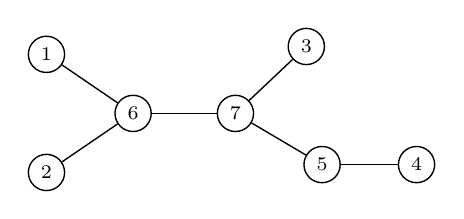
\begin{tikzpicture}[font=\scriptsize,
  pv/.style={circle, draw, line width=0.5pt, inner sep=0pt, minimum size=0.46cm},
  pe/.style={line width=0.5pt}]
\node[pv] (v6) at (0,0) {$6$}; \node[pv] (v1) at (-1.1,0.75) {$1$}; \node[pv] (v2) at (-1.1,-0.75) {$2$};
\node[pv] (v7) at (1.3,0) {$7$}; \node[pv] (v3) at (2.2,0.85) {$3$}; \node[pv] (v5) at (2.4,-0.65) {$5$};
\node[pv] (v4) at (3.6,-0.65) {$4$};
\draw[pe] (v1) -- (v6); \draw[pe] (v2) -- (v6); \draw[pe] (v6) -- (v7); \draw[pe] (v7) -- (v3);
\draw[pe] (v7) -- (v5); \draw[pe] (v5) -- (v4);
\end{tikzpicture}}{A tree with vertex set $\{1,\ldots,7\}$. Its Pr\"ufer code is $(6,6,7,5,7)$ (\cref{tab:prufer}).\label{fig:prufer}}
\end{figure}

\begin{table}
\sdfloat{%
\begin{sdtable}{colspec={cccc}, row{1}={font=\small}}
\toprule
Step & Leaves & Removed & Recorded \\
\midrule
$1$ & $1,2,3,4$ & $1$ & $6$ \\
$2$ & $2,3,4$ & $2$ & $6$ \\
$3$ & $3,4,6$ & $3$ & $7$ \\
$4$ & $4,6$ & $4$ & $5$ \\
$5$ & $5,6$ & $5$ & $7$ \\
\bottomrule
\end{sdtable}}{Computing the Pr\"ufer code of the tree of \cref{fig:prufer}. At each step the smallest leaf is removed and its neighbour recorded. After step~$2$ the vertex $6$ has become a leaf, after step~$4$ the vertex $5$. The edge $67$ remains at the end.\label{tab:prufer}}
\end{table}

\begin{note}{Planar graphs and Euler's formula}
A graph is \term{planar} if it can be drawn in the plane without crossing edges. A drawing of a connected planar graph with $n$ vertices and $m$ edges divides the plane into some number $f$ of regions, the \term{faces}, one of which is unbounded, and Euler's formula states that
\[
n-m+f=2 .
\]
For a tree, $m=n-1$ and $f=1$. A connected plane graph contains a spanning tree (\cref{cor:spanning-tree}), and each of the remaining $m-n+1$ edges, added one at a time, splits one face into two; this gives the formula, the splitting of a face being a consequence of the Jordan curve theorem. Every face of a planar graph with $n\ge3$ vertices is bounded by at least three edges and each edge borders at most two faces, so $3f\le2m$, and Euler's formula yields $m\le3n-6$. Since $K_5$ has $10>3\cdot5-6$ edges, it is not planar. In $K_{3,3}$, which has no triangles, every face is bounded by at least four edges, so $m\le2n-4=8$, whereas $K_{3,3}$ has $9$ edges; so it is not planar either. Kuratowski proved in 1930 that these two graphs are, in a precise sense, the only obstructions: a graph is planar if and only if it contains no subdivision of $K_5$ or $K_{3,3}$~\cite{kuratowski1930}. Diestel gives a careful treatment~\cite[Chap.~4]{diestel2017}, and Aigner and Ziegler present several applications of Euler's formula~\cite{aigner2018proofs}. Planar graphs arise in Volume~XVI as the triangulations used in computational geometry.
\end{note}

\section{Counting and Probability: A First Look}
\label{sec:counting-probability}

Probability began with games of chance, in which a finite number of outcomes, such as the faces of a die, are equally likely. In this setting probability is counting, and this section gives a first look at that connection; Volume~III develops probability theory in general.

\begin{definition}[Classical probability]
\label{def:classical-probability}
Let $\Omega$ be a finite nonempty set, the set of possible \term{outcomes} of an experiment, all of which are assumed to be equally likely. An \term{event} is a subset $E\subseteq\Omega$, and its \term{probability} is
\[
P(E)\coloneqq\frac{|E|}{|\Omega|}.
\]
\end{definition}

This is the definition that Laplace placed at the head of his \emph{Essai philosophique sur les probabilit\'es} of 1814: the probability of an event is the number of favourable cases divided by the number of all possible cases~\cite{laplace1814}. The rules of counting turn into rules of probability. By the sum rule, $P(E\cup F)=P(E)+P(F)$ if $E$ and $F$ are disjoint; by \cref{prop:union-two}, $P(E\cup F)=P(E)+P(F)-P(E\cap F)$ in general, and $P(E\cup F)\le P(E)+P(F)$; and the complement $\Omega\setminus E$ has probability $1-P(E)$. Inclusion--exclusion becomes a formula for the probability of a union of events.

The whole difficulty lies in the choice of $\Omega$: its outcomes must be equally likely. When two dice are thrown, there are eleven possible sums, $2,\ldots,12$, but they are not equally likely. The right model takes as outcomes the $36$ ordered pairs $(i,j)\in\{1,\ldots,6\}^2$, which are equally likely for fair dice thrown independently. The sum $7$ arises from the six pairs $(1,6),(2,5),\ldots,(6,1)$, so its probability is $6/36=1/6$, while the sum $2$ arises only from $(1,1)$ and has probability $1/36$.

\emph{Cards.} A hand of five cards dealt from a well-shuffled deck of $52$ is equally likely to be any of the $\binom{52}5=2\,598\,960$ five-element subsets of the deck. The hands with exactly two aces consist of two of the four aces and three of the $48$ other cards, so by the product rule there are $\binom42\binom{48}3=6\cdot17\,296=103\,776$ of them, and the probability is about $0.0399$. A full house, three cards of one rank and two of another, can be chosen in $13\cdot\binom43\cdot12\cdot\binom42=3744$ ways, which gives the probability $3744/2\,598\,960\approx0.00144$. The first computation is an instance of the hypergeometric distribution, which governs sampling without replacement from a finite population; it reappears in Volume~XIII and in exact tests for contingency tables in Volume~XIV.

\emph{Birthdays.} What is the probability that among $k$ people some two share a birthday? Assume that each of the $365^k$ assignments of birthdays to the $k$ people is equally likely, ignoring leap years. The assignments in which all birthdays differ are the $k$-arrangements of the $365$ days, of which there are $365^{\underline k}$ by \cref{thm:arrangements}. So the probability that all birthdays differ is
\[
q_k=\frac{365^{\underline k}}{365^k}=\prod_{j=1}^{k-1}\Bigl(1-\frac{j}{365}\Bigr),
\]
and the probability of a shared birthday is $1-q_k$. It exceeds $\frac12$ from $k=23$ on, where $1-q_{23}\approx0.507$, and $0.99$ from $k=57$ on. Most people find these numbers surprisingly small~\cite{feller1968}. The explanation is that $k$ people form $\binom k2$ pairs, each of which may share a birthday: $23$ people form $253$ pairs. \Cref{fig:birthday} shows the probability as a function of $k$ together with the approximation $1-e^{-k(k-1)/(2\cdot365)}$, which follows from the inequality $1-t\le e^{-t}$ of Chapter~9 and is a lower bound for it.

\begin{figure}
\sdfloat{%
\begin{tikzpicture}
\begin{axis}[sdplot, width=0.72\textwidth, height=0.4\textwidth, xmin=0, xmax=72, ymin=0, ymax=1.05,
  xtick={0,10,20,23,30,40,50,57,60,70}, xticklabels={0,10,20,,30,40,50,,60,70},
  ytick={0,0.25,0.5,0.75,1}, xlabel={number of people $k$}, ylabel={probability},
  legend style={at={(0.97,0.35)}, anchor=east}]
\addplot[black, densely dotted, line width=0.5pt, forget plot] coordinates {(23,0) (23,0.507297) (0,0.507297)};
\addplot[black, line width=0.7pt, mark=none] coordinates {(1,0.000000) (2,0.002740) (3,0.008204) (4,0.016356) (5,0.027136) (6,0.040462) (7,0.056236) (8,0.074335) (9,0.094624) (10,0.116948) (11,0.141141) (12,0.167025) (13,0.194410) (14,0.223103) (15,0.252901) (16,0.283604) (17,0.315008) (18,0.346911) (19,0.379119) (20,0.411438) (21,0.443688) (22,0.475695) (23,0.507297) (24,0.538344) (25,0.568700) (26,0.598241) (27,0.626859) (28,0.654461) (29,0.680969) (30,0.706316) (32,0.753348) (34,0.795317) (36,0.832182) (38,0.864068) (40,0.891232) (42,0.914030) (44,0.932885) (46,0.948253) (48,0.960598) (50,0.970374) (52,0.978005) (54,0.983877) (56,0.988332) (57,0.990122) (58,0.991665) (60,0.994123) (62,0.995910) (64,0.997190) (66,0.998096) (68,0.998726) (70,0.999160) (72,0.999453)};
\addlegendentry{$1-q_k$}
\addplot[black, dashed, line width=0.7pt, domain=0:72, samples=100] {1-exp(-x*(x-1)/730)};
\addlegendentry{$1-e^{-k(k-1)/730}$}
\end{axis}
\end{tikzpicture}}{The probability $1-q_k$ that among $k$ people two share a birthday (solid), and the approximation $1-e^{-k(k-1)/730}$ (dashed), which lies slightly below it. The dotted lines mark $k=23$, the smallest number of people for which the probability exceeds $\frac12$.\label{fig:birthday}}
\end{figure}

The birthday problem is a problem about collisions, and it has a direct bearing on computing. If $k$ keys are hashed into $N$ slots by a hash function that behaves like a random assignment, the probability that the $k$ keys land in $k$ different slots is $N^{\underline k}/N^k$, and the approximation above shows that a collision becomes more likely than not once $k$ is about $\sqrt{2N\ln2}\approx1.18\sqrt N$. For $N=365$ this gives $22.5$; for hash values of $32$ bits, $N=2^{32}$, it gives about $77\,000$ keys, far fewer than the four billion slots. The same estimate governs the repetition of values drawn at random from a large finite set, for instance by a random number generator (Volume~XIII).

\emph{Matching.} A permutation of $\{1,\ldots,n\}$ chosen uniformly at random is a derangement with probability $D_n/n!$, which by \cref{sec:ie-pigeonhole} is close to $1/e\approx0.368$ for all $n\ge4$ or so. So if $n$ letters are put at random into $n$ addressed envelopes, the probability that no letter reaches its intended recipient is about $37$ per cent, almost independently of $n$.

\emph{Rank sums.} In the example of \cref{sec:gf}, each of the $2^{10}$ subsets of $\{1,\ldots,10\}$ is equally likely when the treatment has no effect, and the probability that the rank sum is at most $8$ is $25/1024\approx0.024$. Exact tests in statistics compute probabilities of this kind by counting, and the counting is often done by the generating functions of \cref{sec:gf}.

Classical probability covers only experiments with finitely many equally likely outcomes. It cannot describe a biased coin, the waiting time until the first success, or a measurement with a continuous range of values. Volume~III builds the general theory on the measure theory of Volume~II; the classical definition survives in it as the uniform distribution on a finite set, and the counting techniques of this chapter remain the tools for computing with it.

\chapternotes

The rules of \cref{sec:counting-principles,sec:perm-comb,sec:binomial} are treated in every textbook of discrete mathematics. Graham, Knuth and Patashnik~\cite{graham1994concrete} cover binomial coefficients, recurrences, finite calculus, special numbers and generating functions with an eye to the analysis of algorithms, and the first volume of Knuth's \emph{The Art of Computer Programming}~\cite{knuth1997taocp1} contains a compact and careful account of the same material (Sections~1.2.5--1.2.9). For a broader view, van Lint and Wilson~\cite{vanlint2001} survey combinatorics in short chapters, and Stanley~\cite{stanley2012ec1} is the standard advanced text on enumeration; its first chapter organises the counting problems of \cref{tab:four-ways} and their relatives into the ``twelvefold way'', and its second chapter treats inclusion--exclusion. Aigner and Ziegler~\cite{aigner2018proofs} collect particularly elegant proofs, among them the pigeonhole and double counting arguments of \cref{sec:ie-pigeonhole} and four proofs of Cayley's formula.

Wilf's \emph{generatingfunctionology}~\cite{wilf2006} is a readable introduction to generating functions, and Flajolet and Sedgewick~\cite{flajolet2009} develop them into a systematic method for counting combinatorial structures and estimating the counts asymptotically. Andrews~\cite{andrews1976partitions} is the standard reference on partitions, and Stanley's monograph on Catalan numbers~\cite{stanley2015catalan} contains their history and more than two hundred interpretations. Feller's classic introduction to probability~\cite{feller1968} uses combinatorial arguments throughout, including the birthday problem, the matching problem of \cref{sec:counting-probability} and the reflection principle.

For graph theory, West~\cite{west2001} is a comprehensive undergraduate text, Bondy and Murty~\cite{bondymurty2008} and Diestel~\cite{diestel2017} are standard graduate texts, and Biggs, Lloyd and Wilson~\cite{biggs1976} reprint and comment on the original papers from Euler's bridges to K\H{o}nig's book, including Cayley's work on trees. Graham, Rothschild and Spencer~\cite{graham1990ramsey} introduce Ramsey theory. The algorithmic side of graphs and trees, from traversal and shortest paths to spanning trees and union--find, is the subject of Cormen, Leiserson, Rivest and Stein~\cite{cormen2022} and of Volume~IV.

\chapterreferences
